\documentclass{article}
\usepackage{graphicx}
\graphicspath{{recursos/}}

% cor das caixas
\usepackage{xcolor}
\definecolor{vermelho}{RGB}{224,25,26}

% fontes de texto e ambiente matemático
\usepackage{avant}
\usepackage{mathptmx}

% pacotes de configuração
\usepackage{config/estrutura/headers}
\usepackage[corlink=vermelho]{config/estrutura/fontes}
\usepackage[cor=vermelho]{config/estrutura/ambientes}
\usepackage{config/estrutura/margens}
\usepackage[cor=vermelho]{config/estrutura/secoes}
\usepackage[logo=logo.png]{config/estrutura/titulo}

% pacotes extras
\usepackage{caption, subcaption, pdfpages, wrapfig}
\usepackage{circuitikz, graphics, float}

% começa a seção no `0`
\setcounter{section}{-1}



\hypersetup{
    pdftitle  = {Gráficos no Origin},
    pdfauthor = {Tiago de Paula}
}

\title{Criação e Formatação de Gráficos com o}\softwarelogo
\author{\href{mailto:t187679@dac.unicamp.br}{Tiago de Paula}}
\date{}


\begin{document}
    \maketitle

    O \software é um dos \textit{softwares} mais tradicionais e mais robustos na área de análise gráfica de dados. Inicialmente foi densenvolvido para ser usado com microcalorímetros, mas seu foco foi mudando para áres de pesquisa em geral e suas funcionalidades acompanharam, se tornando cada vez mais genérica. Por se tratar de um produto pago, a sua qualidade é bem confiável e vem recheados com as mais variadas ferramentas para desenhar gráficos e analisar os dados envolvidos.

    Nesse tutorial, no entanto, serão abordadas apenas as ferramentas necessárias para o curso de Física Experimental 3 (\texttt{F 329}). O tutorial parte das funcionalidades mais básicas, nas duas primeiras seções (\nameref{sec:basico} e \nameref{sec:reta}), que serão usadas em todos os gráficos, até algumas partes um pouco mais específicas, de \nameref{sec:escala}, \nameref{sec:caract}, \nameref{sec:multiv} e \nameref{sec:contorno}. As outras seções, \nameref{sec:regres} e \nameref{sec:incert}, que são intermediárias, também serão usadas em vários gráficos de vários experimentos distintos.

    \section{Configurações Básicas} \label{sec:basico}
        \begin{figure}[H]
    \centering
    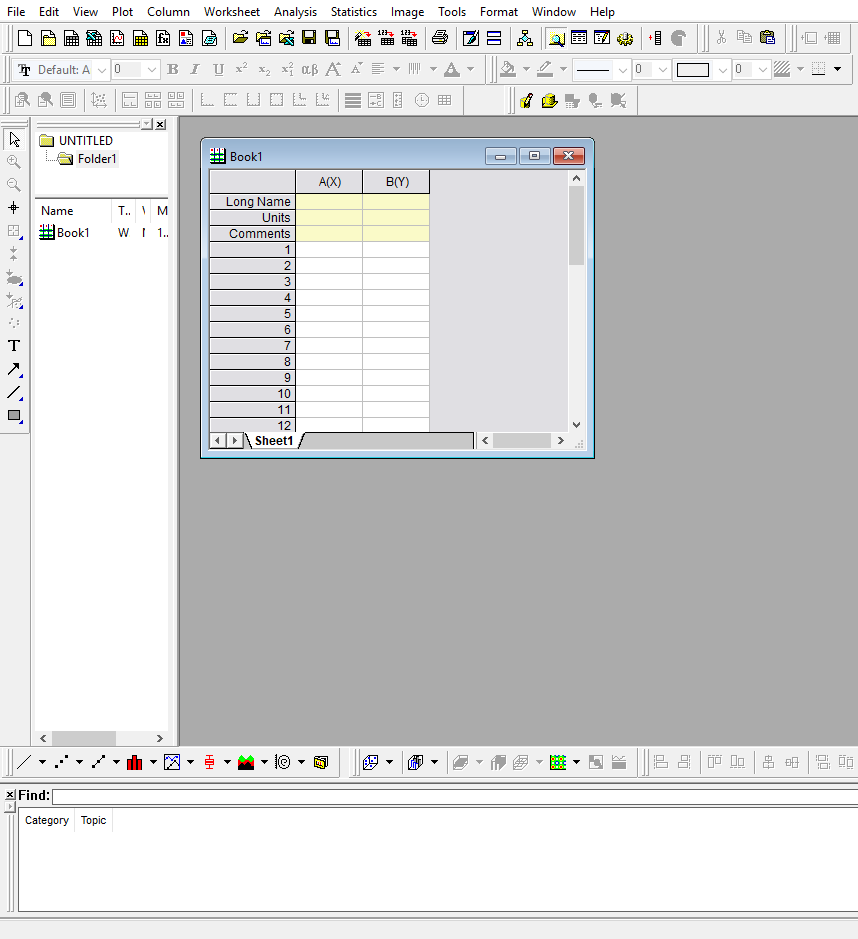
\includegraphics[width=0.7\textwidth]{basico/1mostra.png}

    \caption{Tela inicial do Origin}
    \label{fig:basico:mostragem}
\end{figure}

\subsection{Alterando a Fonte Padrão}

    Como a fonte padrão do \software não funciona muito bem com acentos e outros símbolos da língua portuguesa, é recomendado utilizar outra fonte nos gráficos. Nos exemplos a seguir será aplicada a fonte \texttt{Times New Roman}, que funciona com os acentos gráficos e é facilmente encontrada em qualquer máquina com \texttt{Windows}. Todo o processo é bem simples e está especificado na figura \ref{fig:basico:mudar_fontes}.

    \begin{figure}[htbp]
        \centering
        \begin{subfigure}{0.45\textwidth}
            \centering
            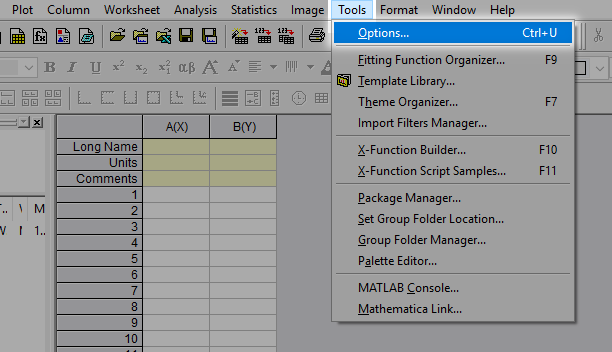
\includegraphics[width=\textwidth]{basico/2options.png}

            \caption{Acesso às opções}
            \label{fig:basico:options}
        \end{subfigure}
        ~
        \begin{subfigure}{0.45\textwidth}
            \centering
            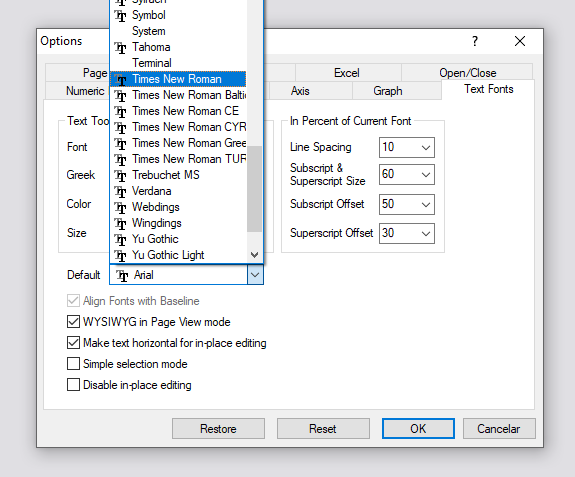
\includegraphics[width=\textwidth]{basico/3fonts.png}

            \caption{Opção de fontes}
            \label{fig:basico:fontes}
        \end{subfigure}
        \caption{Mudando a fonte padrão}
        \label{fig:basico:mudar_fontes}
    \end{figure}


\subsection{Importando os Dados}

    Os dados podem ser apenas copiados de um gerenciador de tabelas como o \texttt{Excel}, o \texttt{Google Planilhas} ou o \\\texttt{LibreOffice Calc} e colados na tabela do \software. Quando os dados são importados assim, a formatação das linhas e colunas se matém.

    Também é possível importar dados de arquivos de texto, como os arquivos com extensão \texttt{.csv} ou planilhas salvas do \texttt{Excel}, apesar de ser um pouco mais complicado. Versões mais recentes do programa fornecem até a opção de pegar dados de páginas da \textit{internet}.

    \begin{lembrete}
        Cuidado com o separador decimal. Em português e outras línguas europeias é mais comum encontrar a vírgula [\texttt{,}] como separador da parte decimal do número, enquanto nos países anglofônicos é o ponto final [\texttt{.}] que define a parte fracionária e a vírgula serve para separar os milhares. Isso pode trazer problemas na hora de importar os dados, dependendo da configuração do \software e da formatação original dos dados.
    \end{lembrete}


\subsection{Renomeando Colunas} \label{sec:basico:renome}

    Por padrão, as colunas são criadas com letras (figura \ref{fig:basico:importado}). Para mudar isso, basta alterar as propriedades da coluna (acessada com um clique duplo na coluna), como na figura \ref{fig:basico:renomear}. Os campos mais importantes são:

    \begin{description}
        \item[Short Name] o nome da coluna na tabela do \software
        \item[Long Name] um nome mais descritivo para o valor e é o que normalmente aparece no gráfico
        \item[Units] a gradeza física do valor
        \item[Plot Designation] é a função da coluna no gráfico, que pode ser \texttt{Y}, \texttt{X}, \texttt{YErr}, \texttt{Z}, entre outros...
    \end{description}

    Além disso, se você importar os dados de um arquivo \texttt{CSV}, é possível utilizar as primeiras linhas como nome ou descrição da coluna.

    \begin{figure}[htbp]
        \centering
        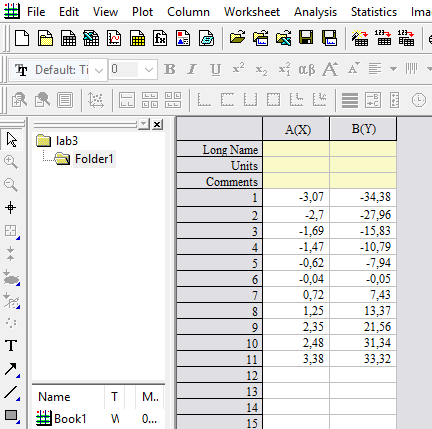
\includegraphics[width=0.7\textwidth]{basico/4import.png}

        \caption{Colunas com nomes genérico}
        \label{fig:basico:importado}
    \end{figure}

    \begin{figure}[htbp]
        \centering
        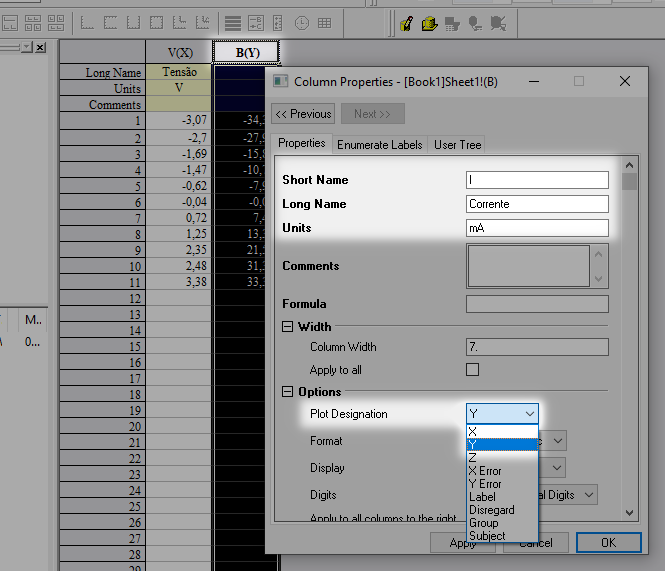
\includegraphics[width=0.8\textwidth]{basico/5renome.png}

        \caption{Alterando as propriedades da coluna}
        \label{fig:basico:renomear}
    \end{figure}


    \section{Apresentação dos Dados} \label{sec:reta}
        Nesta seção, será tomado como exemplo a relação de corrente e tensão em um resistor, dado pela teoria por (\ref{eq:resist}). São os mesmos dados da figura \ref{fig:basico:importado}, da seção \nameref{sec:basico}, que foram gerados por computador.

\begin{equacao} \label{eq:resist}
    I = \frac{1}{R} ~ V
\end{equacao}

Por mais que sejam esses os dados usados aqui, essa parte de apresentação de dados é importante para todos dados, em especial, quando coletados à mão, como é o caso dos experimentos da disciplina de \texttt{F 329}.


\subsection{Dados Pontuais}

    Normalmente, quando se trata de dados pontuais, é importante mostrar esses dados em alguma tabela e no gráfico também. O modo de se fazer isso no \texttt{Origin} é com a funcionalidade \texttt{Scatter} (figura \ref{fig:reta:scatter}).

    \begin{figure}[htbp]
        \centering
        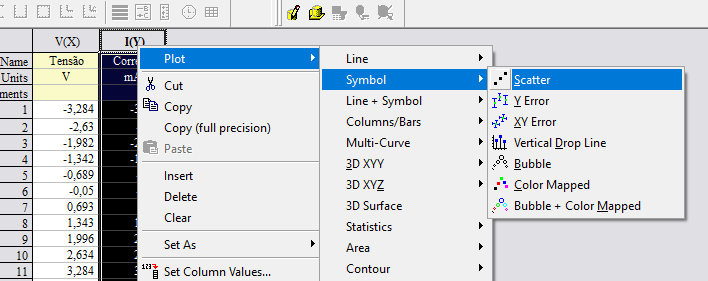
\includegraphics[width=0.7\textwidth]{reta/1scatter.png}

        \caption{\texttt{Scatter}}
        \label{fig:reta:scatter}
    \end{figure}

    \begin{figure}[htbp]
        \centering
        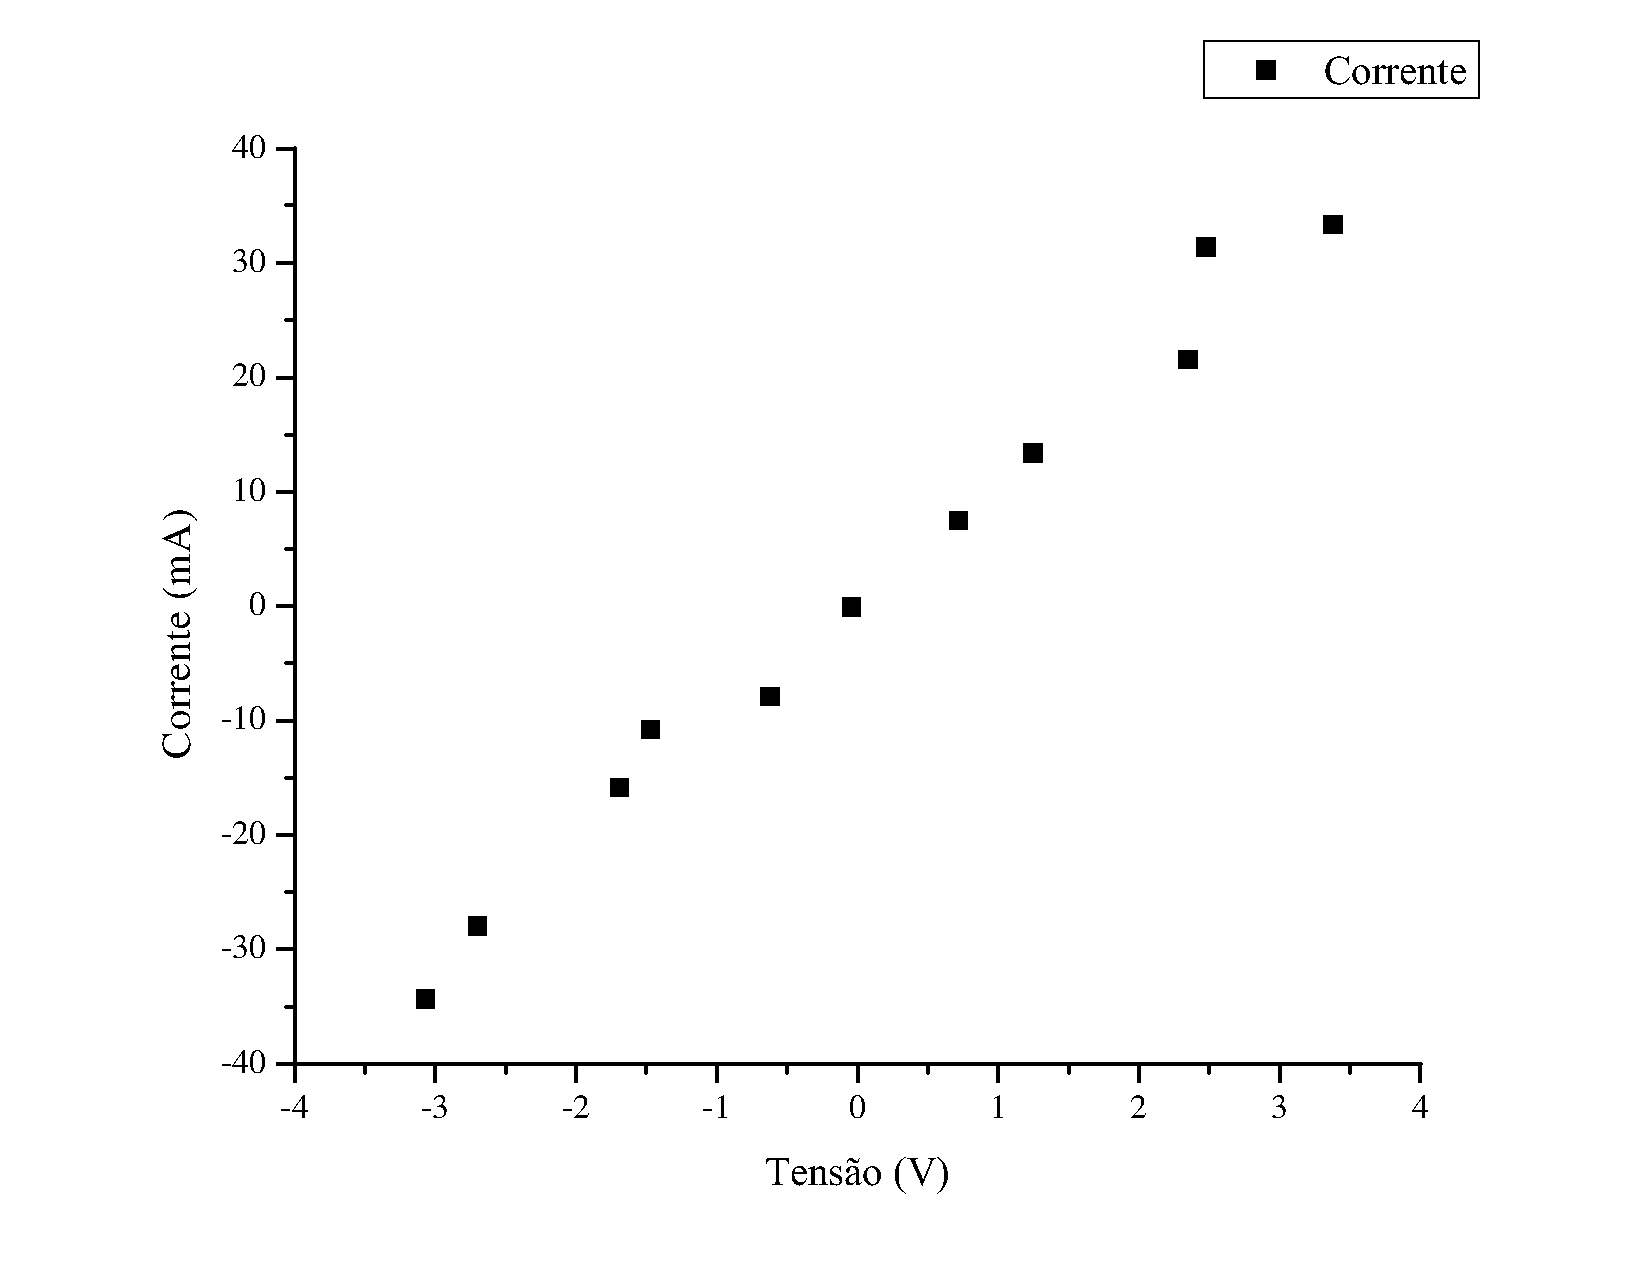
\includegraphics[width=0.8\textwidth]{reta/1linscatter.pdf}

        \caption{Resultado do \texttt{Scatter}}
        \label{fig:reta:linscatter}
    \end{figure}


\subsection{Tratamento da Legenda}

    O \texttt{Origin} gera uma legenda padrão para os elementos desenhados no gráfico. O ideal é alterá-las para serem mais informativas. As legendas também podem ser reposicionadas apenas arrastando-as.

    \begin{figure}[htbp]
        \centering
        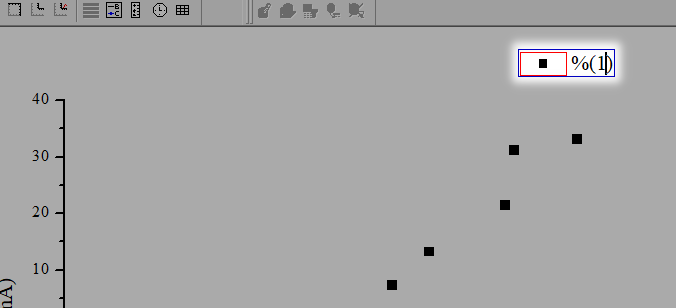
\includegraphics[width=0.8\textwidth]{reta/2legenda.png}

        \caption{Alterando o texto da legenda}
        \label{fig:reta:logenda}
    \end{figure}


\subsection{Marcadores de Ponto}

    Os pontos de dados do \texttt{Scatter} são por padrão marcados com um quadrado preenchido. Isso pode ser alterado acessando as opções por qualquer um dos pontos no gráfico. Existem várias opções de formatação do marcador, incluindo desenho, tamanho e cor.

    \begin{figure}[htbp]
        \centering
        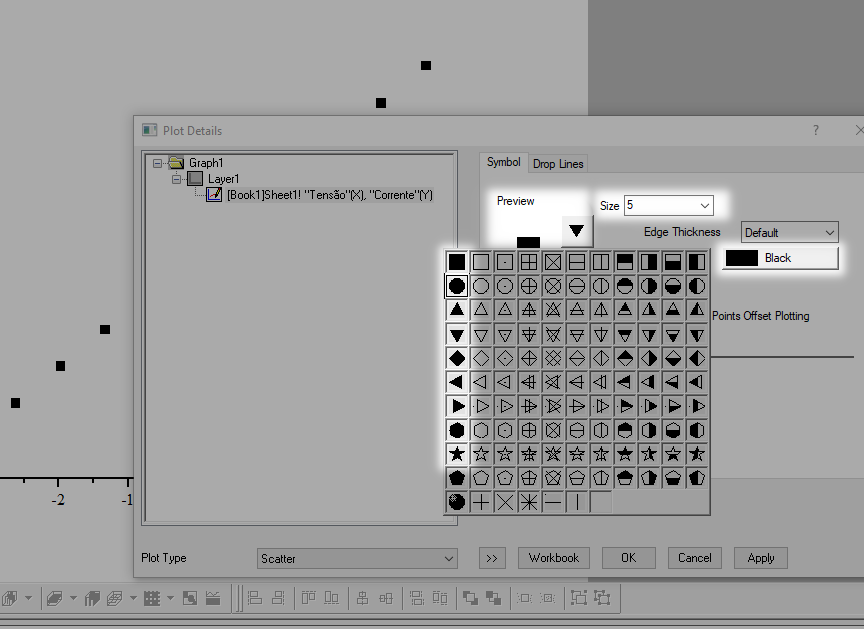
\includegraphics[width=0.8\textwidth]{reta/3marks.png}

        \caption{Alterando os marcadores}
        \label{fig:reta:marcadores}
    \end{figure}

    No material, será usado marcadores circulares, preenchidos com preto e de tamanho 5.


\subsection{Linhas de Grid}

    Para ler melhor os eixos do gráfico, é possível colocar retas acompanhando os valores principais.

    \begin{figure}[htbp]
        \centering
        \begin{subfigure}{0.25\textwidth}
            \centering
            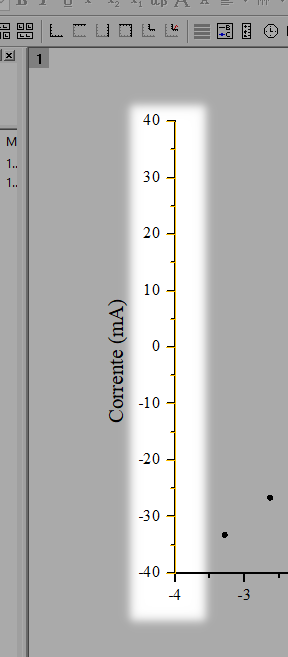
\includegraphics[width=\textwidth]{reta/4eixos.png}

            \caption{Acesso às opções dos eixos}
            \label{fig:reta:eixos}
        \end{subfigure}
        ~
        \begin{subfigure}{0.7\textwidth}
            \centering
            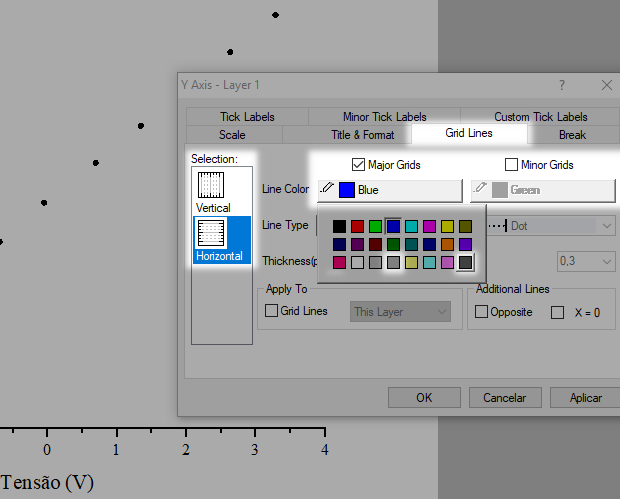
\includegraphics[width=\textwidth]{reta/5grid.png}

            \caption{Opções dos eixos (aba \texttt{Grid Lines})}
            \label{fig:reta:grid}
        \end{subfigure}
        \caption{Opções de linhas de \textit{grid}}
        \label{fig:reta:opcoes_eixo}
    \end{figure}

    No material, será utilizado linhas horizontais e verticais. As linhas principais serão em cinza escuro em traços e as linhas secundárias em cinza claro com pontilhado. Essas configurações podem e devem ser alteradas para cada gráfico, dependendo da importância da leitura dos valores.

    \begin{figure}[htbp]
        \centering
        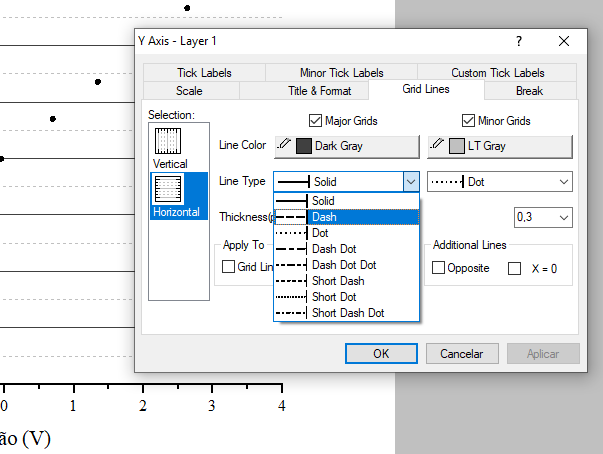
\includegraphics[width=0.8\textwidth]{reta/6gridtipo.png}

        \caption{Colocando e formatando as linha de acompanhamento dos eixos}
        \label{fig:reta:gridtipo}
    \end{figure}


\subsection{Resultado}

    \begin{figure}[htbp]
        \centering
        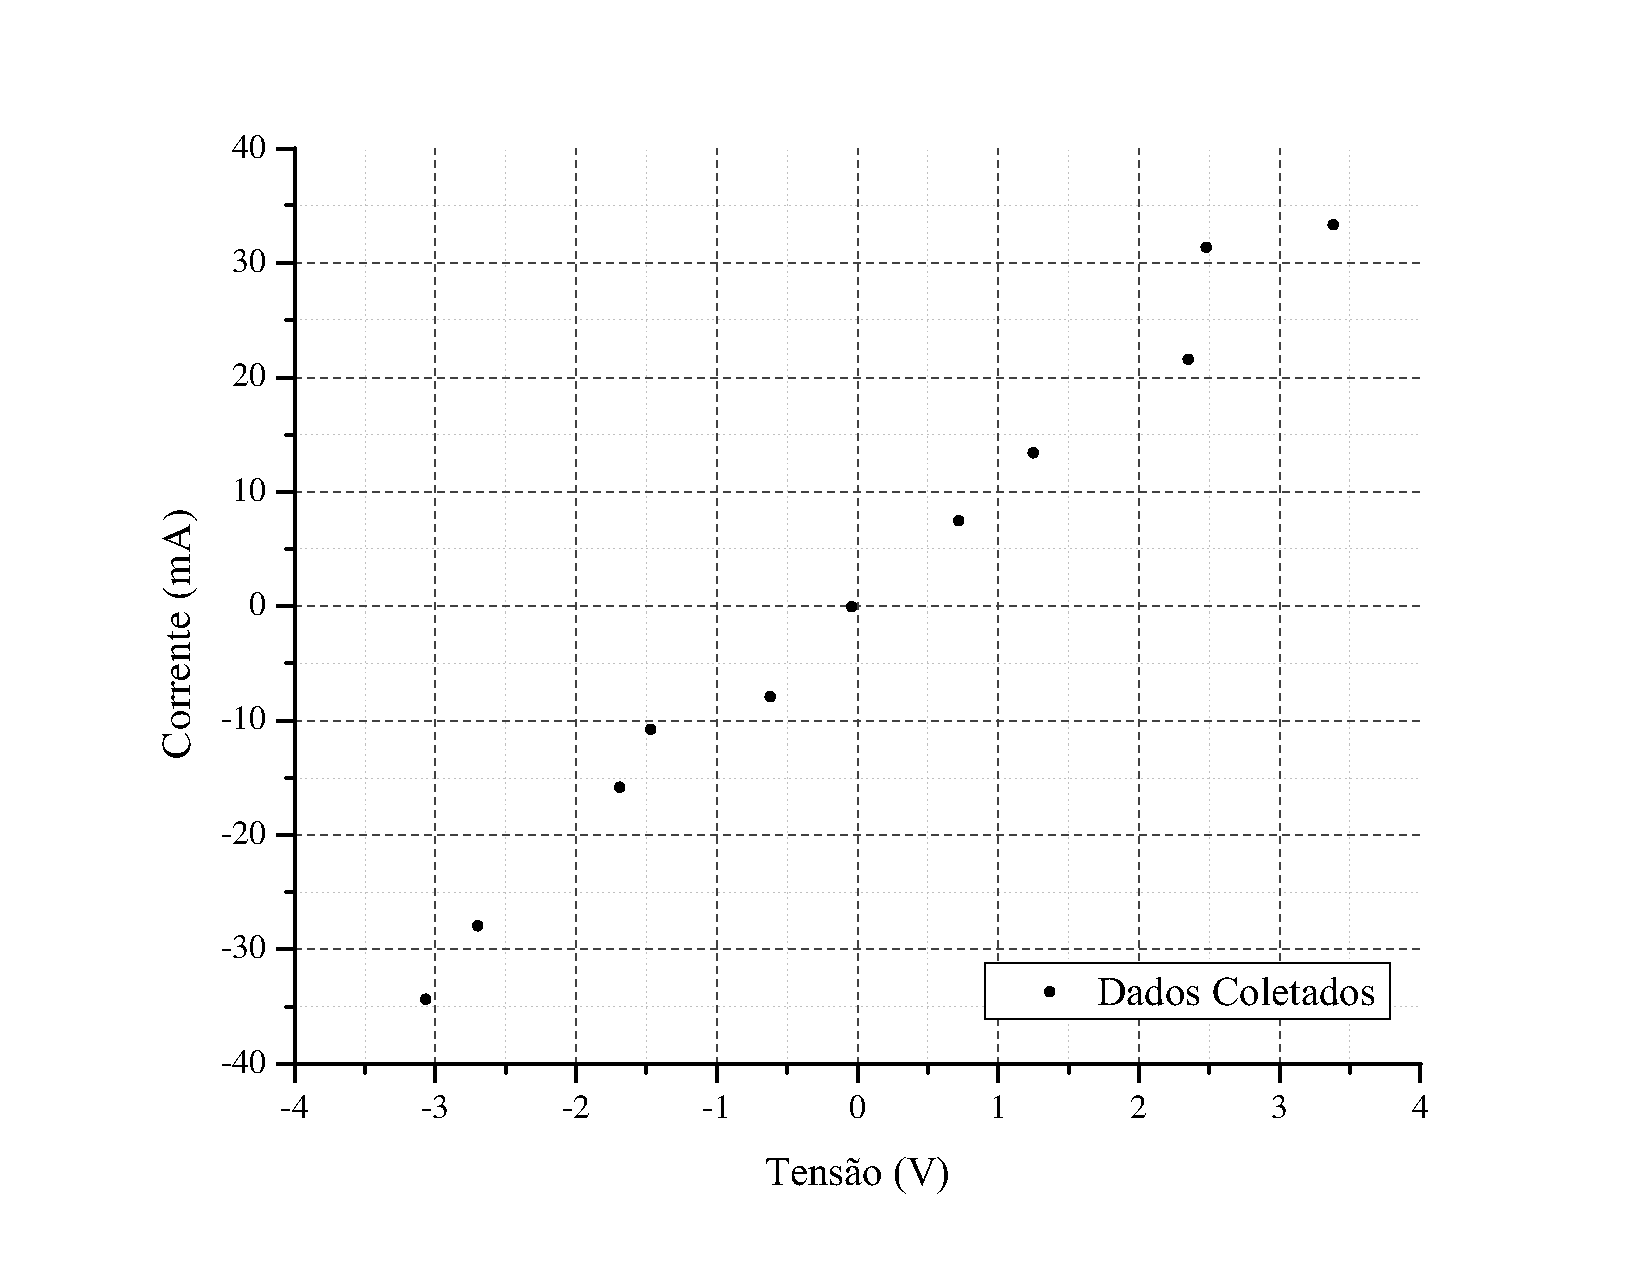
\includegraphics[width=0.8\textwidth]{reta/2gridlinscat.pdf}

        \caption{Gráfico de exemplo dos valores de corrrente e de tensão}
        \label{fig:reta:gridlinscat}
    \end{figure}



    \section{Regressão Linear} \label{sec:regres}
        É muito comum aparecer algum tipo de relação linear entre os dados. Nesse tipo de relação costuma-se aplicar técnicas de regressão, normalmente mínimos quadrados, para encontrar a melhor reta que representa esses dados.

Pelo alinhamento dos pontos da seção \nameref{sec:reta} e pela equação teórica \ref{eq:resist}, fica clara a possibilidade de se aplicar uma regressão linear e, portanto, os dados continuarão os mesmos nessa seção.

\subsection{Configuração da Regressão}

    A regressão normalmente é feita pelas opções \textbf{Analysis: Fitting: Fit Linear}. Isso abre a janela de opções (figura \ref{fig:regres:opt}). Quando terminada a regressão, aparecerá uma janela perguntando para mudar de aba, mas por enquanto é melhor continuar nesta aba.

    Existem outras formas de regressão além da linear, mas elas não serão abordadas nesta matéria.

    \begin{figure}[htbp]
        \centering
        \begin{subfigure}{0.60\textwidth}
            \centering
            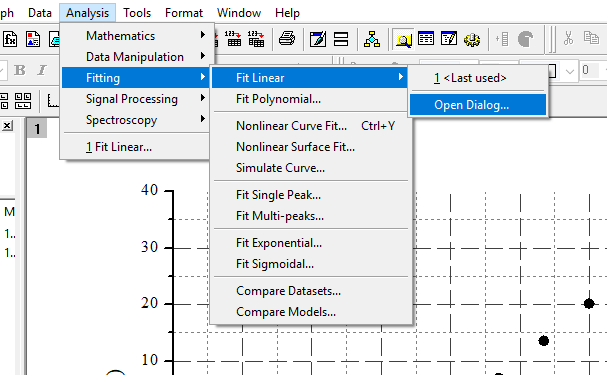
\includegraphics[width=\textwidth]{regres/1regpath.png}

            \caption{Acessando as opções de regressão}
            \label{fig:regres:path}
        \end{subfigure}
        ~
        \begin{subfigure}{0.35\textwidth}
            \centering
            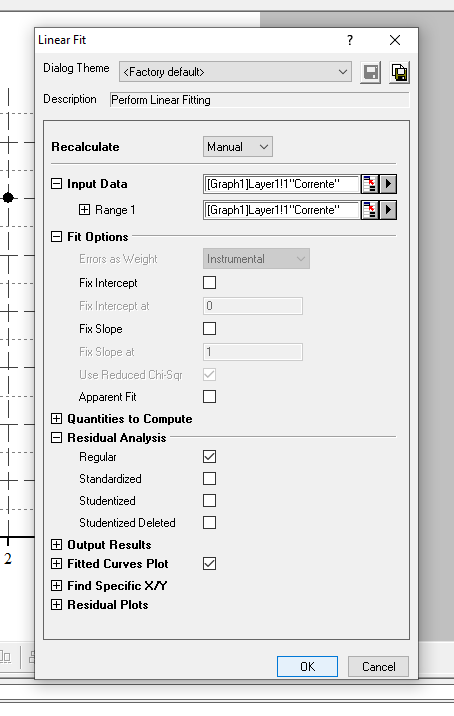
\includegraphics[width=\textwidth]{regres/2regopt.png}

            \caption{Opções de regressão}
            \label{fig:regres:opt}
        \end{subfigure}
        \caption{Configuração da regressão}
        \label{fig:regres:config}
    \end{figure}


    \subsection{Tabela dos Coeficientes}

    Por padrão, os coeficientes da regressão aparecem na tabela como está na figura \ref{fig:regres:coefspadrao}. Ao acessar a tabela \texttt{Table1} na parte esquerda do programa, é possível modificar essa tabela. Após a modificação, é importante apertar \texttt{Update Table} para atualizar a visualização no gráfico.

    \begin{figure}[htbp]
        \centering
        \begin{subfigure}{0.45\textwidth}
            \centering
            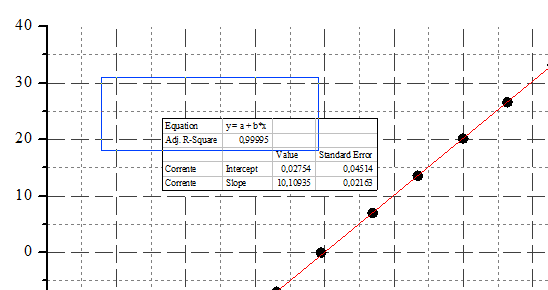
\includegraphics[width=\textwidth]{regres/4mover.png}

            \caption{Tabela padrão de coeficientes da regressão}
            \label{fig:regres:coefspadrao}
        \end{subfigure}
        ~
        \begin{subfigure}{0.50\textwidth}
            \centering
            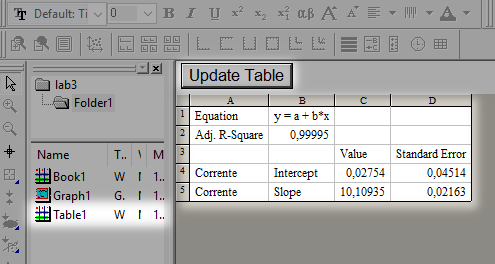
\includegraphics[width=\textwidth]{regres/5tabcoefs.png}

            \caption{Configuração da tabela de coeficientes}
            \label{fig:regres:tabcoefs}
        \end{subfigure}
        \caption{Tabela de coeficientes da regressão}
        \label{fig:regres:coefs}
    \end{figure}


\subsection{Formatação dos Coeficientes}

    Por padrão, os coeficientes da regressão aparecem na tabela como está na figura \ref{fig:regres:coefspadrao}. Ao acessar a aba \texttt{Table1} na parte esquerda do programa, é possível modificar essa tabela.

    Na figura \ref{fig:regres:renome2}, aparece o padrão que será seguido neste tutorial para essa tabela de coeficientes. As dimensões da tabela (figura \ref{fig:regres:tamanhos}), que mudam para cada caso, não seguirão nenhum padrão aqui.

    \begin{figure}[htbp]
        \centering
        \begin{subfigure}{0.45\textwidth}
            \centering
            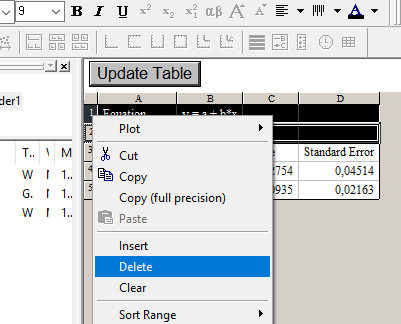
\includegraphics[width=\textwidth]{regres/6del1.png}

            \caption{Removendo as linhas superiores}
            \label{fig:regres:del1}
        \end{subfigure}
        ~
        \begin{subfigure}{0.450\textwidth}
            \centering
            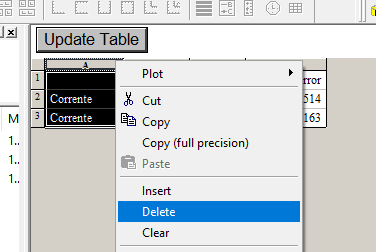
\includegraphics[width=\textwidth]{regres/7del2.png}

            \caption{Removendo as colunas de descrição}
            \label{fig:regres:del2}
        \end{subfigure}
        \caption{Reduzindo a tabela de coeficientes}
        \label{fig:regres:del}
    \end{figure}

    \begin{figure}[htbp]
        \centering
        \begin{subfigure}{0.45\textwidth}
            \centering
            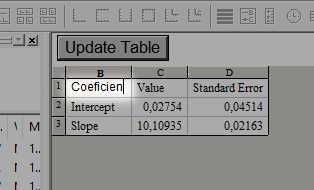
\includegraphics[width=\textwidth]{regres/8renome.png}

            \caption{Renomeando os campos}
            \label{fig:regres:renome1}
        \end{subfigure}
        ~
        \begin{subfigure}{0.450\textwidth}
            \centering
            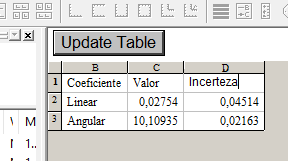
\includegraphics[width=\textwidth]{regres/9renomeado.png}

            \caption{Campos da tabela depois de renomeados}
            \label{fig:regres:renome2}
        \end{subfigure}
        \caption{Renomeando os campos da tabela de coeficientes da regressão}
        \label{fig:regres:renome}
    \end{figure}

    \begin{figure}[htbp]
        \centering
        \begin{subfigure}{0.5\textwidth}
            \centering
            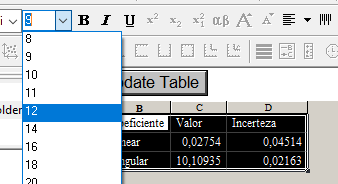
\includegraphics[width=\textwidth]{regres/10fontetam.png}

            \caption{Ajustando o tamanho da fonte}
            \label{fig:regres:fontetam}
        \end{subfigure}
        ~
        \begin{subfigure}{0.40\textwidth}
            \centering
            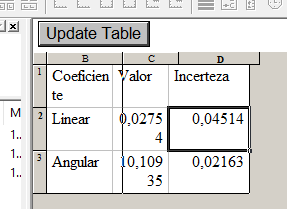
\includegraphics[width=\textwidth]{regres/11colunatam.png}

            \caption{Ajustando a largura da coluna}
            \label{fig:regres:colunatam}
        \end{subfigure}
        \caption{Ajustando as dimensões da tabela de coeficientes da regressão}
        \label{fig:regres:tamanhos}
    \end{figure}

    \begin{figure}[htbp]
        \centering
        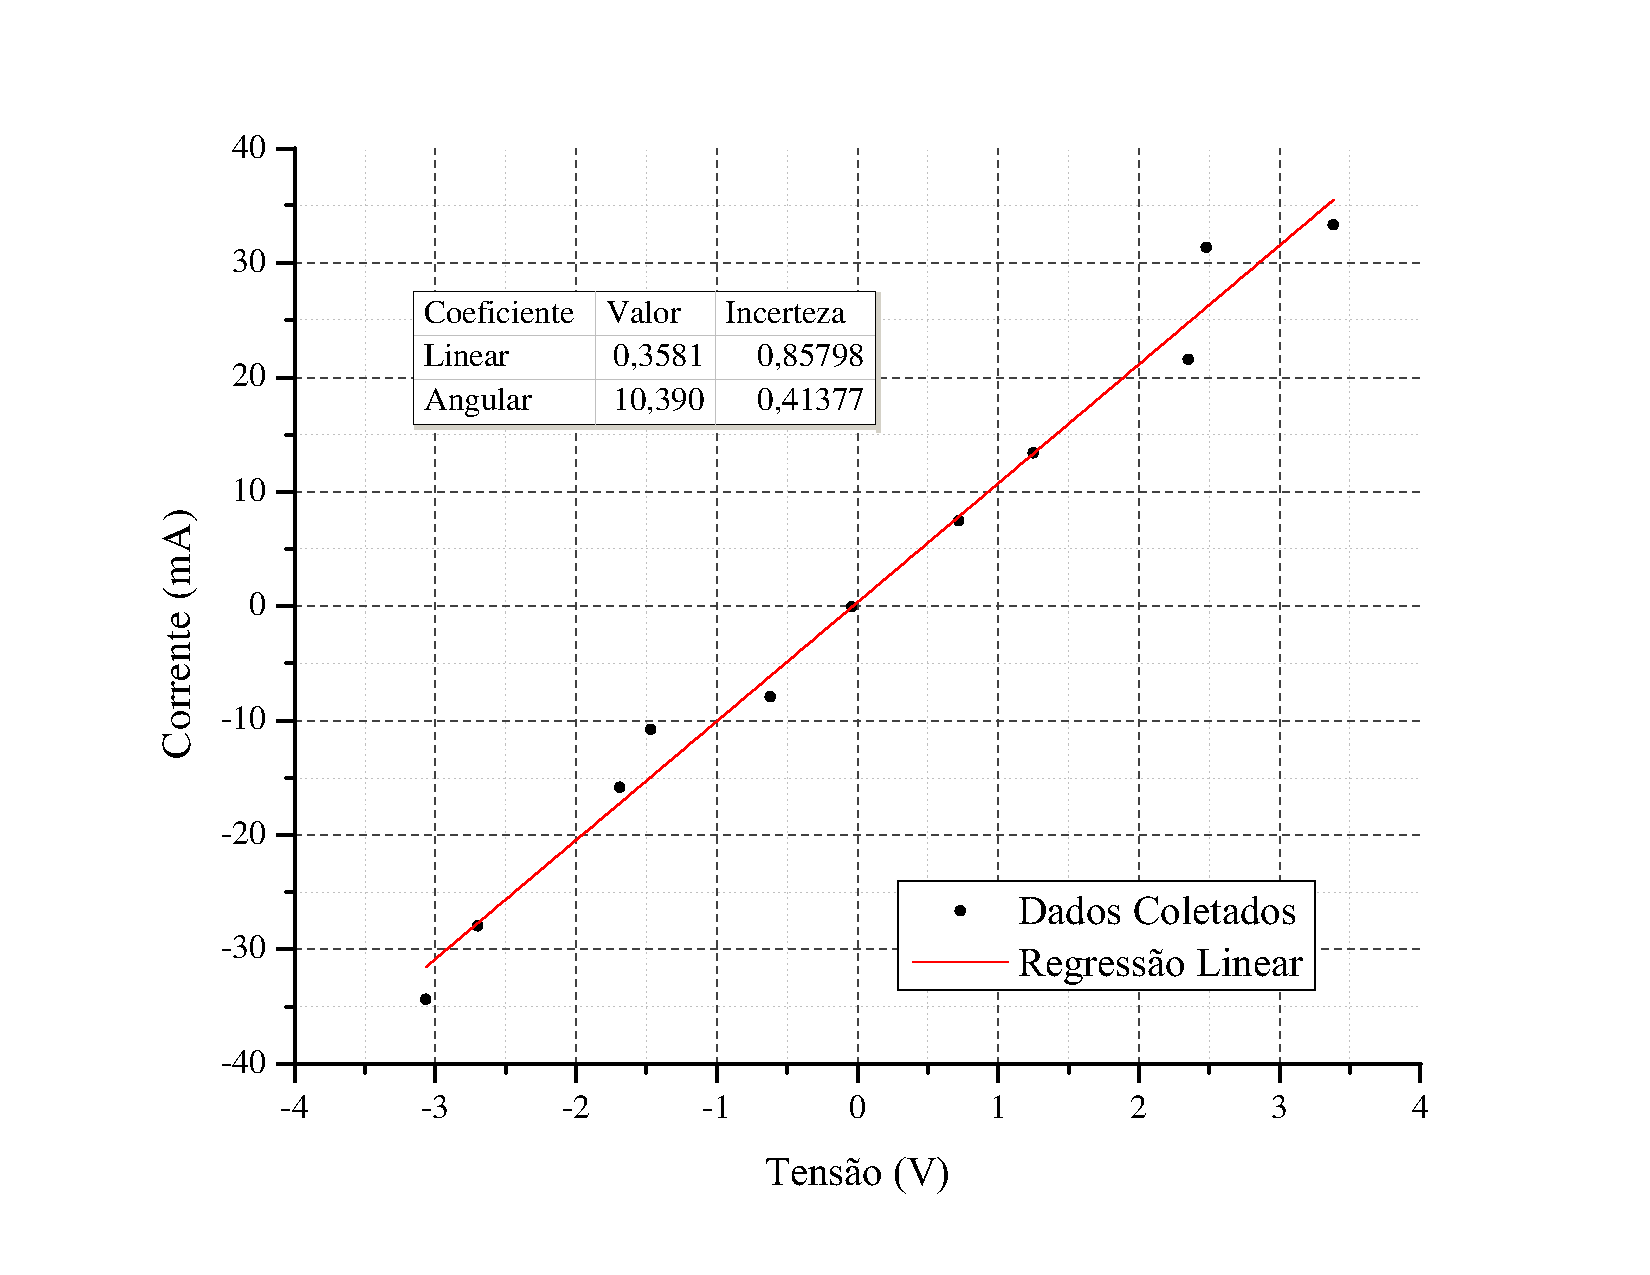
\includegraphics[width=0.8\textwidth]{regres/z1parcial.pdf}

        \caption{Exemplo de regressão linear para a relação de corrrente por tensão}
        \label{fig:regres:semifinal}
    \end{figure}


\subsection{Pontos Fora da Reta}

    Podemos ver que a regressão (figura \ref{fig:regres:semifinal}) resultou em alguns pontos que não ficaram muito próximos a reta encontradada. Esses pontos podem ser marcados para serem ignorados na regressão, como mostra a figura \ref{fig:regres:outliers}. Note que os pontos marcados passam a ser coloridos em vermelho (figura \ref{fig:regres:recalc}).

    \begin{figure}[htbp]
        \centering
        \begin{subfigure}{0.35\textwidth}
            \centering
            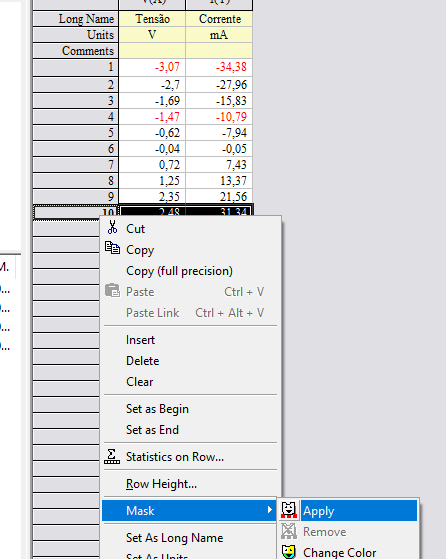
\includegraphics[width=\textwidth]{regres/12remov.png}

            \caption{Marcando os pontos a serem ignorados}
            \label{fig:regres:mask}
        \end{subfigure}
        ~
        \begin{subfigure}{0.35\textwidth}
            \centering
            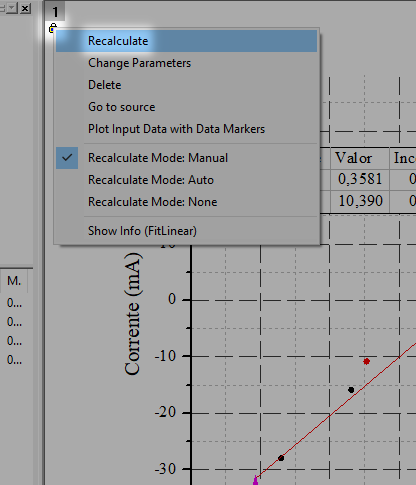
\includegraphics[width=\textwidth]{regres/13recalc.png}

            \caption{Recalculando os coeficientes da regressão}
            \label{fig:regres:recalc}
        \end{subfigure}
        \caption{Removendo pontos selecionados da regressão}
        \label{fig:regres:outliers}
    \end{figure}


\subsection{Resultado}

    \begin{figure}[htbp]
        \centering
        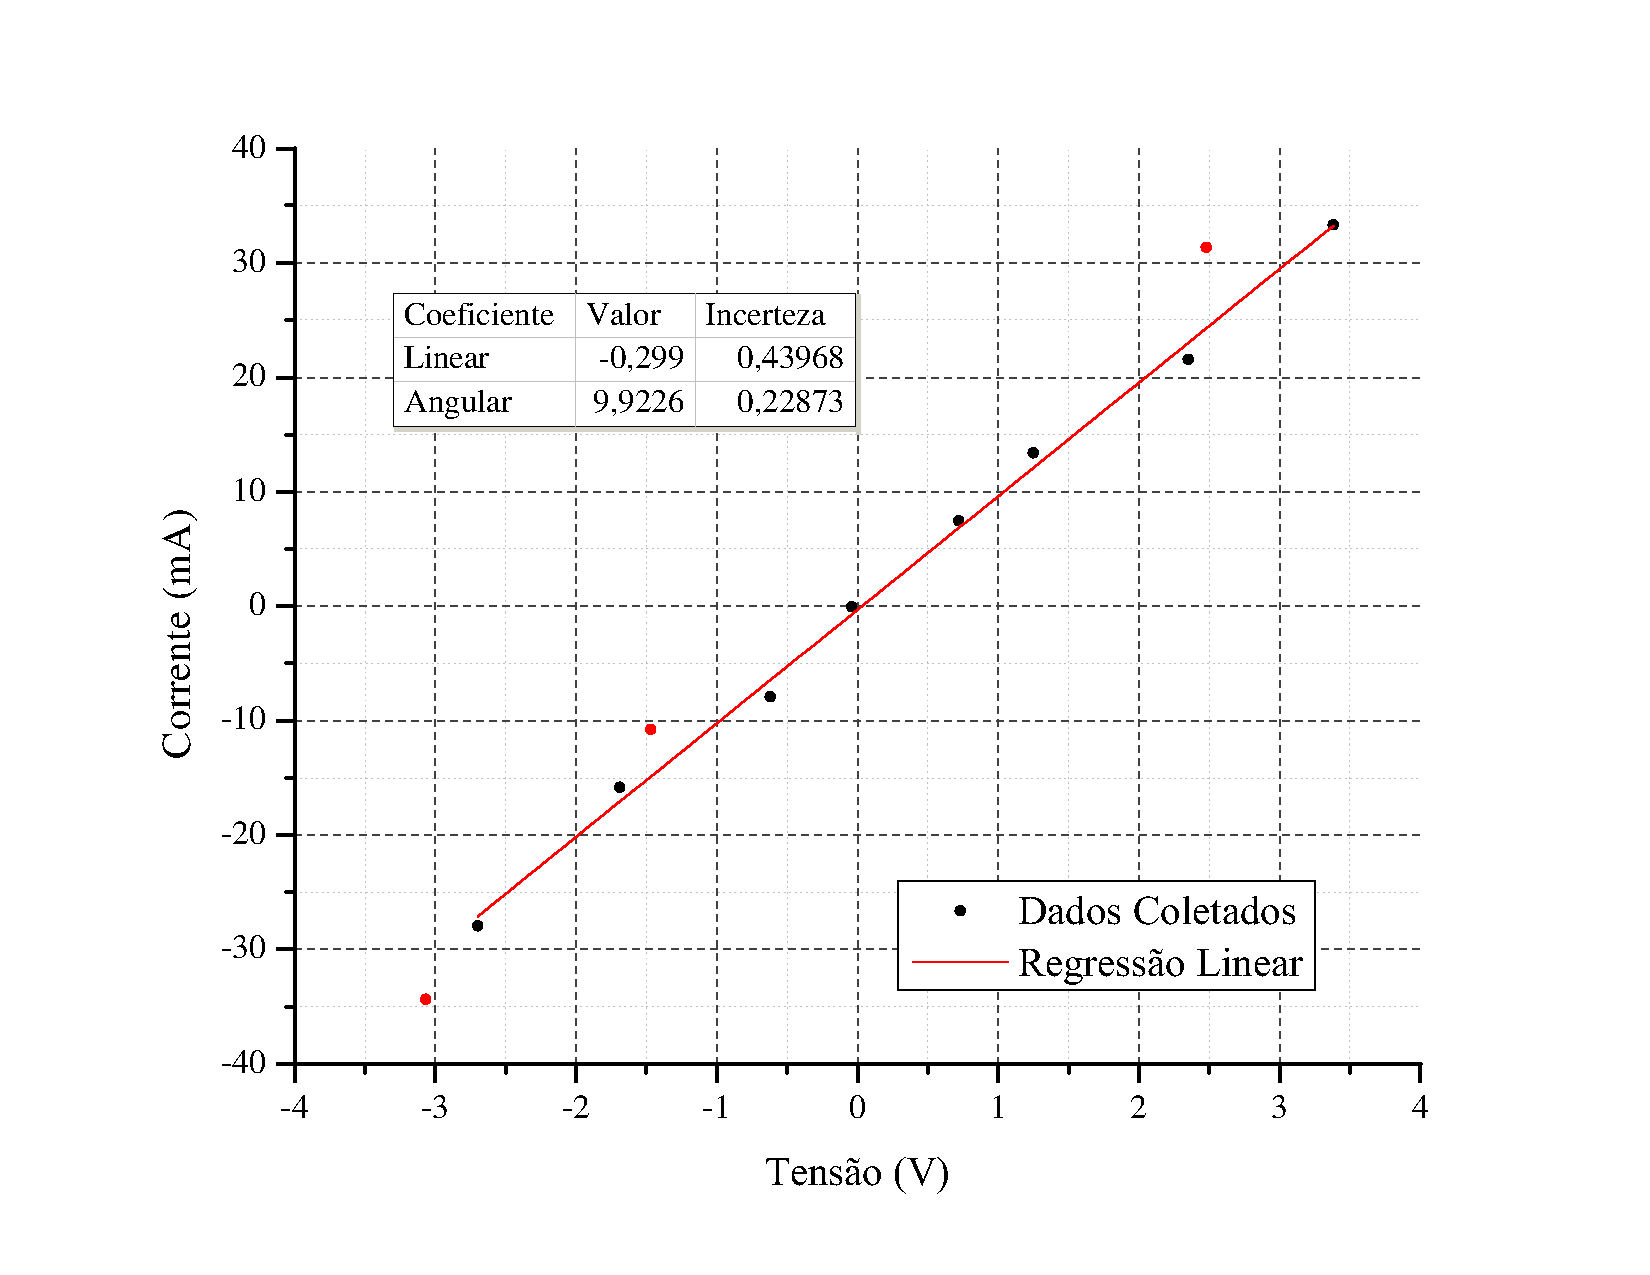
\includegraphics[width=0.8\textwidth]{regres/z2final.pdf}

        \caption{Exemplo de regressão linear com pontos ignorados}
        \label{fig:regres:final}
    \end{figure}

    Observando o resultado na figura \ref{fig:regres:final}, a nova regressão com os pontos ignorados obteve uma redução significativa na incerteza dos coeficientes. Isso indica que a remoção de \textit{outliers} é um passo importante na medição, mas deve ser feito com cuidado. A retirada de pontos válidos para a regressão pode reduzir não só a exatidão da medida, mas até mesmo a precisão, pela maneira como o cálculo da regressão é feito.


    \section{Barras de Incerteza} \label{sec:incert}
        Como exemplo para a aplicação de barras de incerteza, continuaremos com os mesmo dados da seção \nameref{sec:reta}, porém agora com as incertezas associadas a cada medida, que, foram criadas, novamente, com o auxílio de um computador.


\subsection{Adicionando Colunas}

    \begin{figure}[htbp]
        \centering
        \begin{subfigure}{0.27\textwidth}
            \centering
            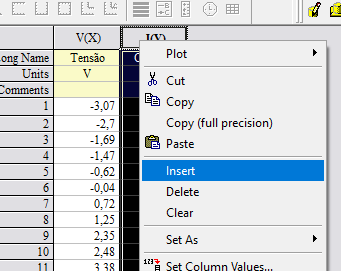
\includegraphics[width=\textwidth]{incert/1insert.png}

            \caption{Inserindo novas colunas}
            \label{fig:incert:insert}
        \end{subfigure}
        ~
        \begin{subfigure}{0.35\textwidth}
            \centering
            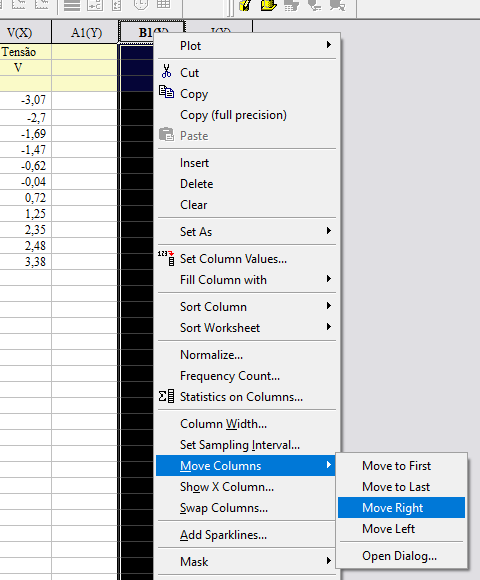
\includegraphics[width=\textwidth]{incert/2move.png}

            \caption{Mudando a posição das colunas}
            \label{fig:incert:mover}
        \end{subfigure}
        \caption{Criando novas colunas}
        \label{fig:incert:colunas}
    \end{figure}

    Para adicionar a incertezas, é preciso gerar novas colunas nas tabelas, como mostra a figura \ref{fig:incert:colunas}, lembrando sempre de formatá-las como na seção \nameref{sec:basico:renome}. A tabela com os dados de incerteza deve ficar algo parecido com a figura \ref{fig:incert:dados}.

    \begin{figure}[htbp]
        \centering
        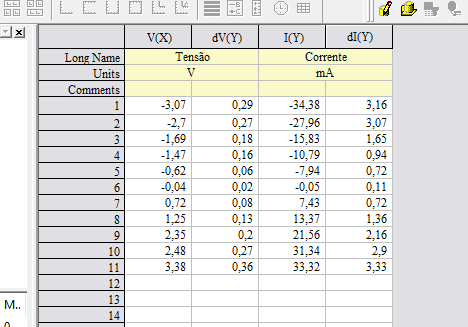
\includegraphics[width=0.7\textwidth]{incert/3dados.png}

        \caption{Dados atualizados com as incertezas}
        \label{fig:incert:dados}
    \end{figure}


\subsection{Tipo das Novas Colunas}

    \begin{figure}[htbp]
        \centering
        \begin{subfigure}{0.45\textwidth}
            \centering
            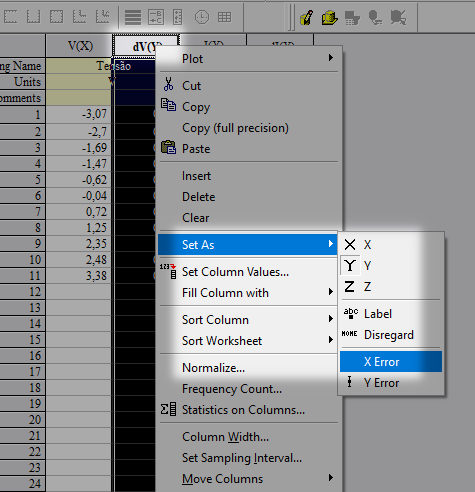
\includegraphics[width=\textwidth]{incert/4xer.png}

            \caption{Incerteza em \texttt{X}}
            \label{fig:incert:xer}
        \end{subfigure}
        ~
        \begin{subfigure}{0.45\textwidth}
            \centering
            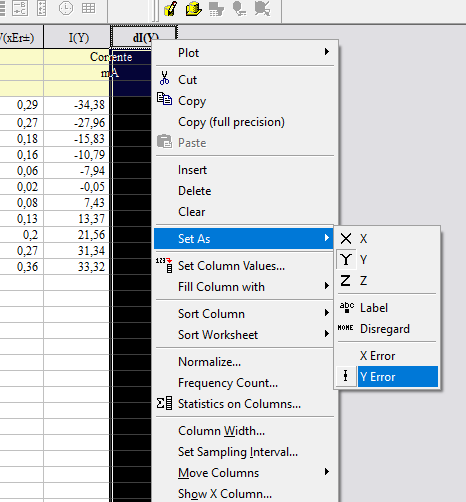
\includegraphics[width=\textwidth]{incert/5yer.png}

            \caption{Incerteza em \texttt{Y}}
            \label{fig:incert:yer}
        \end{subfigure}
        \caption{Mudando o tipo das novas colunas para relacionar com os valores das medidas}
        \label{fig:incert:tipos}
    \end{figure}


\subsection{Formatação das Barras de Incerteza}

    As barras de incerteza também têm várias configurações de formatação relacionadas a elas, mas aqui só será alterado o tamanho do traço final da barra (em inglês, \textit{cap}) como exemplo na figura \ref{fig:incert:capsz}.

    \begin{figure}[htbp]
        \centering
        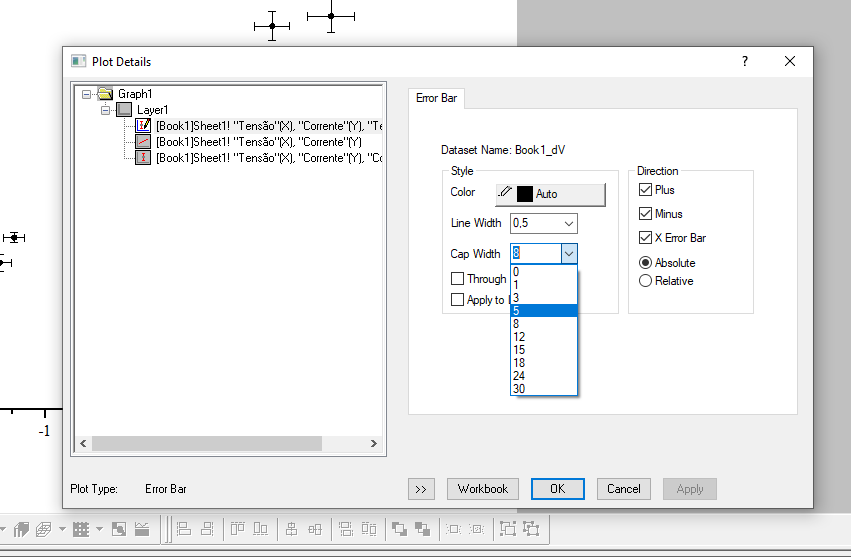
\includegraphics[width=0.7\textwidth]{incert/6cap.png}

        \caption{Dados atualizados com as incertezas}
        \label{fig:incert:capsz}
    \end{figure}


\subsection{Resultados}

    A funcionalidade \texttt{Scatter}, quando selecionada com as colunas de incerteza, gera o gráfico da figura \ref{fig:incert:preresultado}.

    \begin{figure}[htbp]
        \centering
        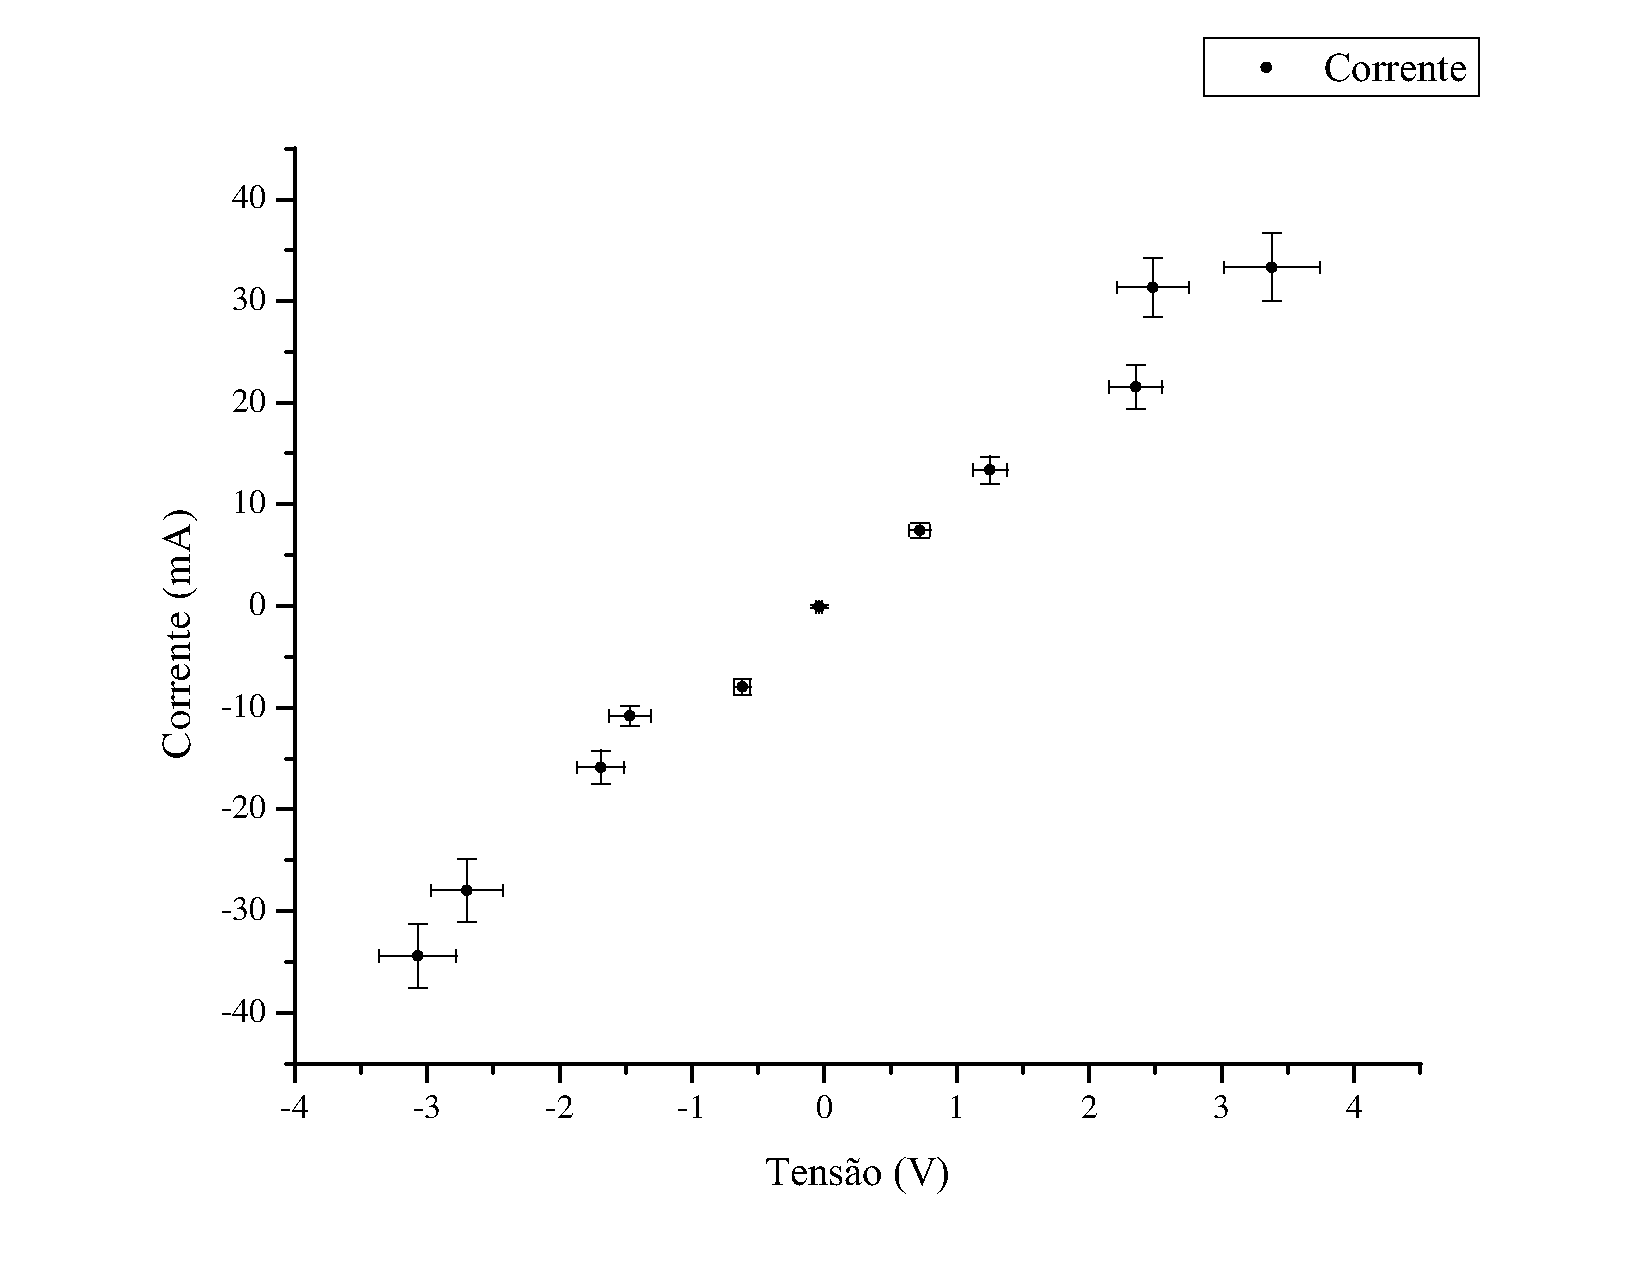
\includegraphics[width=0.8\textwidth]{incert/preresultado.pdf}

        \caption{Gráfico de corrrente por tensão com as incertezas de cada medida}
        \label{fig:incert:preresultado}
    \end{figure}

    Entretanto, se for aplicada a formatação da seção \nameref{sec:reta} e a regressão linear, como na seção \nameref{sec:regres}, o resultado deveria ficar semelhante a figura \ref{fig:incert:resultado}.

    \begin{figure}[htbp]
        \centering
        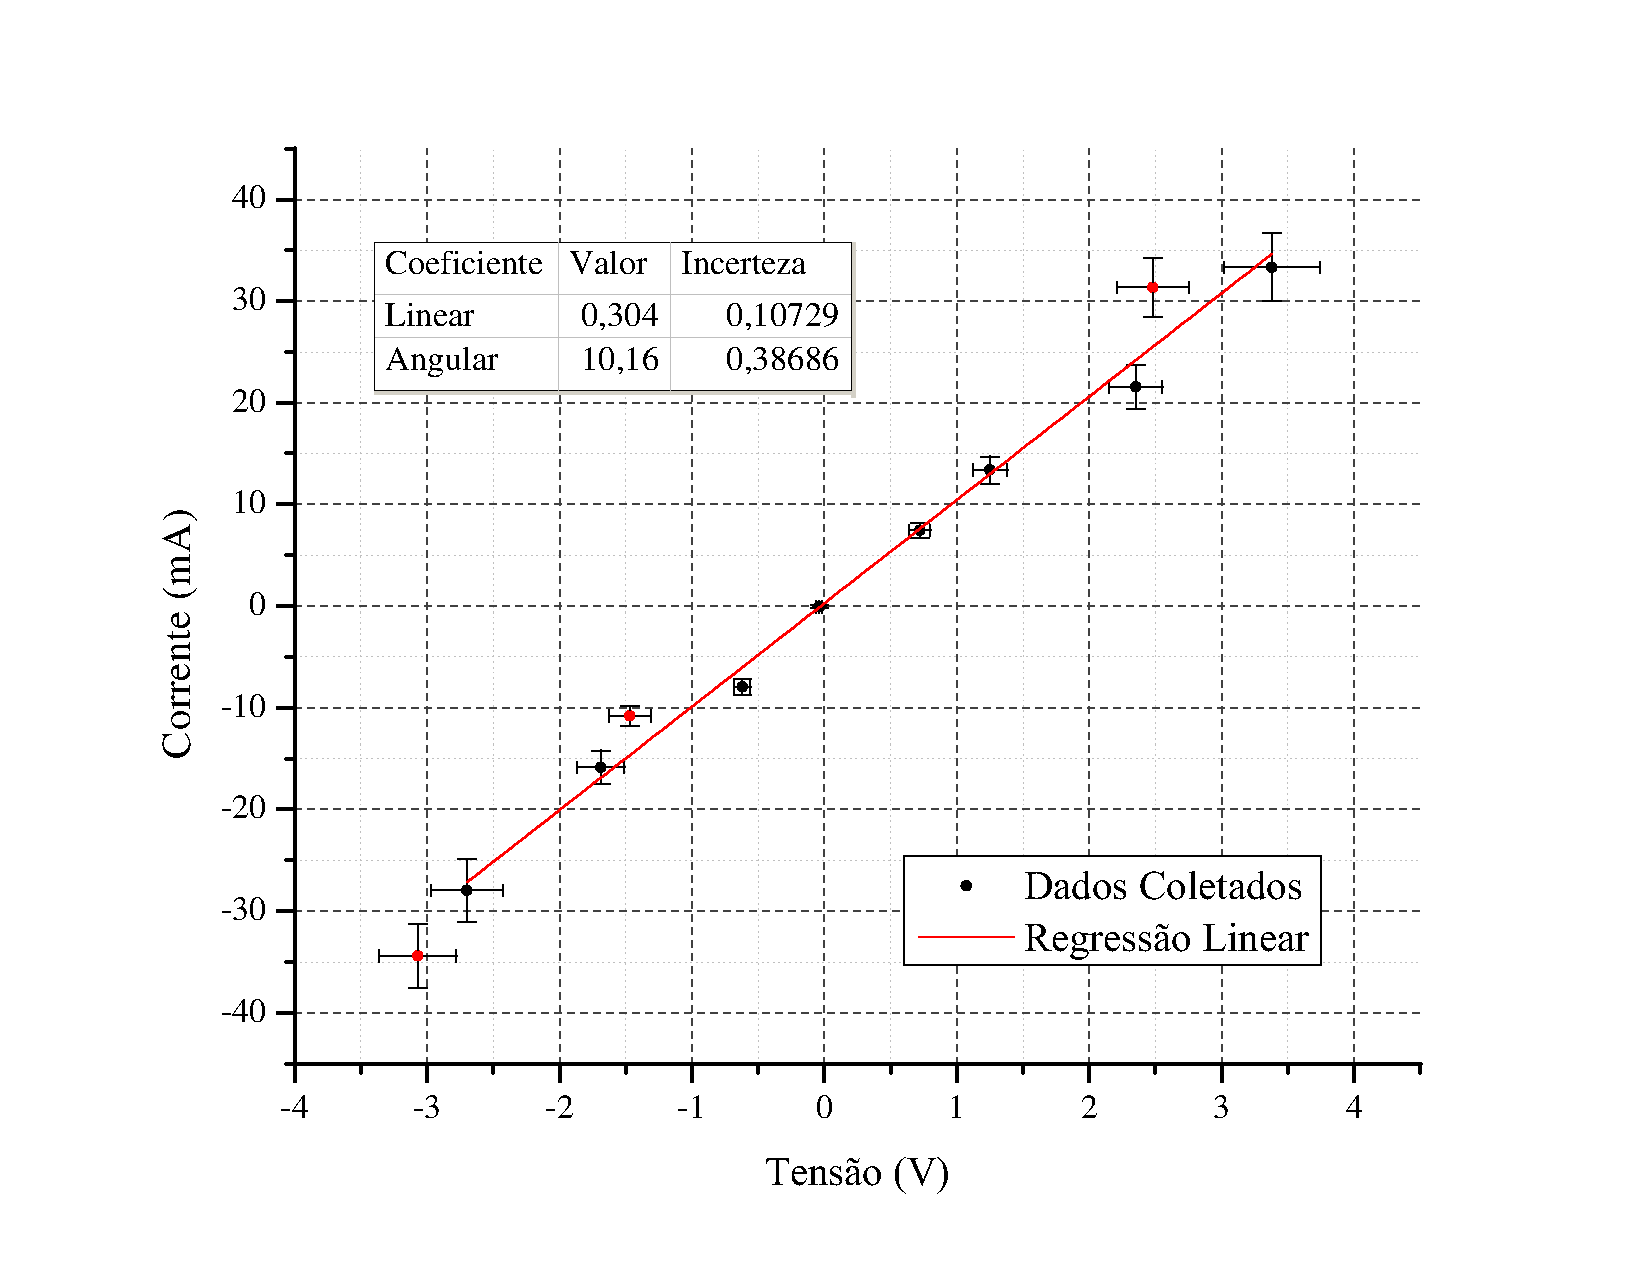
\includegraphics[width=0.8\textwidth]{incert/resultado.pdf}

        \caption{Gráfico formatado, com barras de incerteza e regressão linear}
        \label{fig:incert:resultado}
    \end{figure}

    \begin{nota}
        Note que os coeficientes da regressão em \ref{fig:incert:resultado}, tanto os valores quanto as incertezas, são levemente diferentes da figura \ref{fig:regres:final}, até mesmo com dados numéricos idênticos. A diferença aqui se deve as incertezas dos dados, que agora estão sendo levadas em conta no cálculo da regressão.

        Na verdade, apenas a incerteza em \texttt{Y} está sendo levada em conta. A regressão com as incertezas de \texttt{X} só estão presentes nas versões mais novas do \texttt{Origin}.
    \end{nota}


    \section{Escala Logarítmica} \label{sec:escala}
        Várias vezes, no entanto, os dados não apresentam relação linear. Nesses casos, é importante encontrar alguma técnica de linearização que transforma os dados para novos valores dependentes, mas que se relacionam de maneira linear. Algo como a relação (\ref{eq:linearizacao}).

\begin{equacao} \label{eq:linearizacao}
    f(x, y) = a + b ~ g(x, y)
\end{equacao}

Dentre as técnicas mais comuns, muitas envolvem a aplicação de logaritmos para linearizar alguma relação de potência de $x$, isto é, nos casos de $y \propto x^k$, ou alguma relação exponencial, $y \propto k^x$. Para esses casos, é comum a utilização de escala logarítmica na intenção de se observar melhor os dados, em que $f(x, y) = \log(y)$ e $g(x, y) = \log(x)$.


\subsection{Gráfico Log-Log}

    \begin{figure}[htbp]
        \centering
        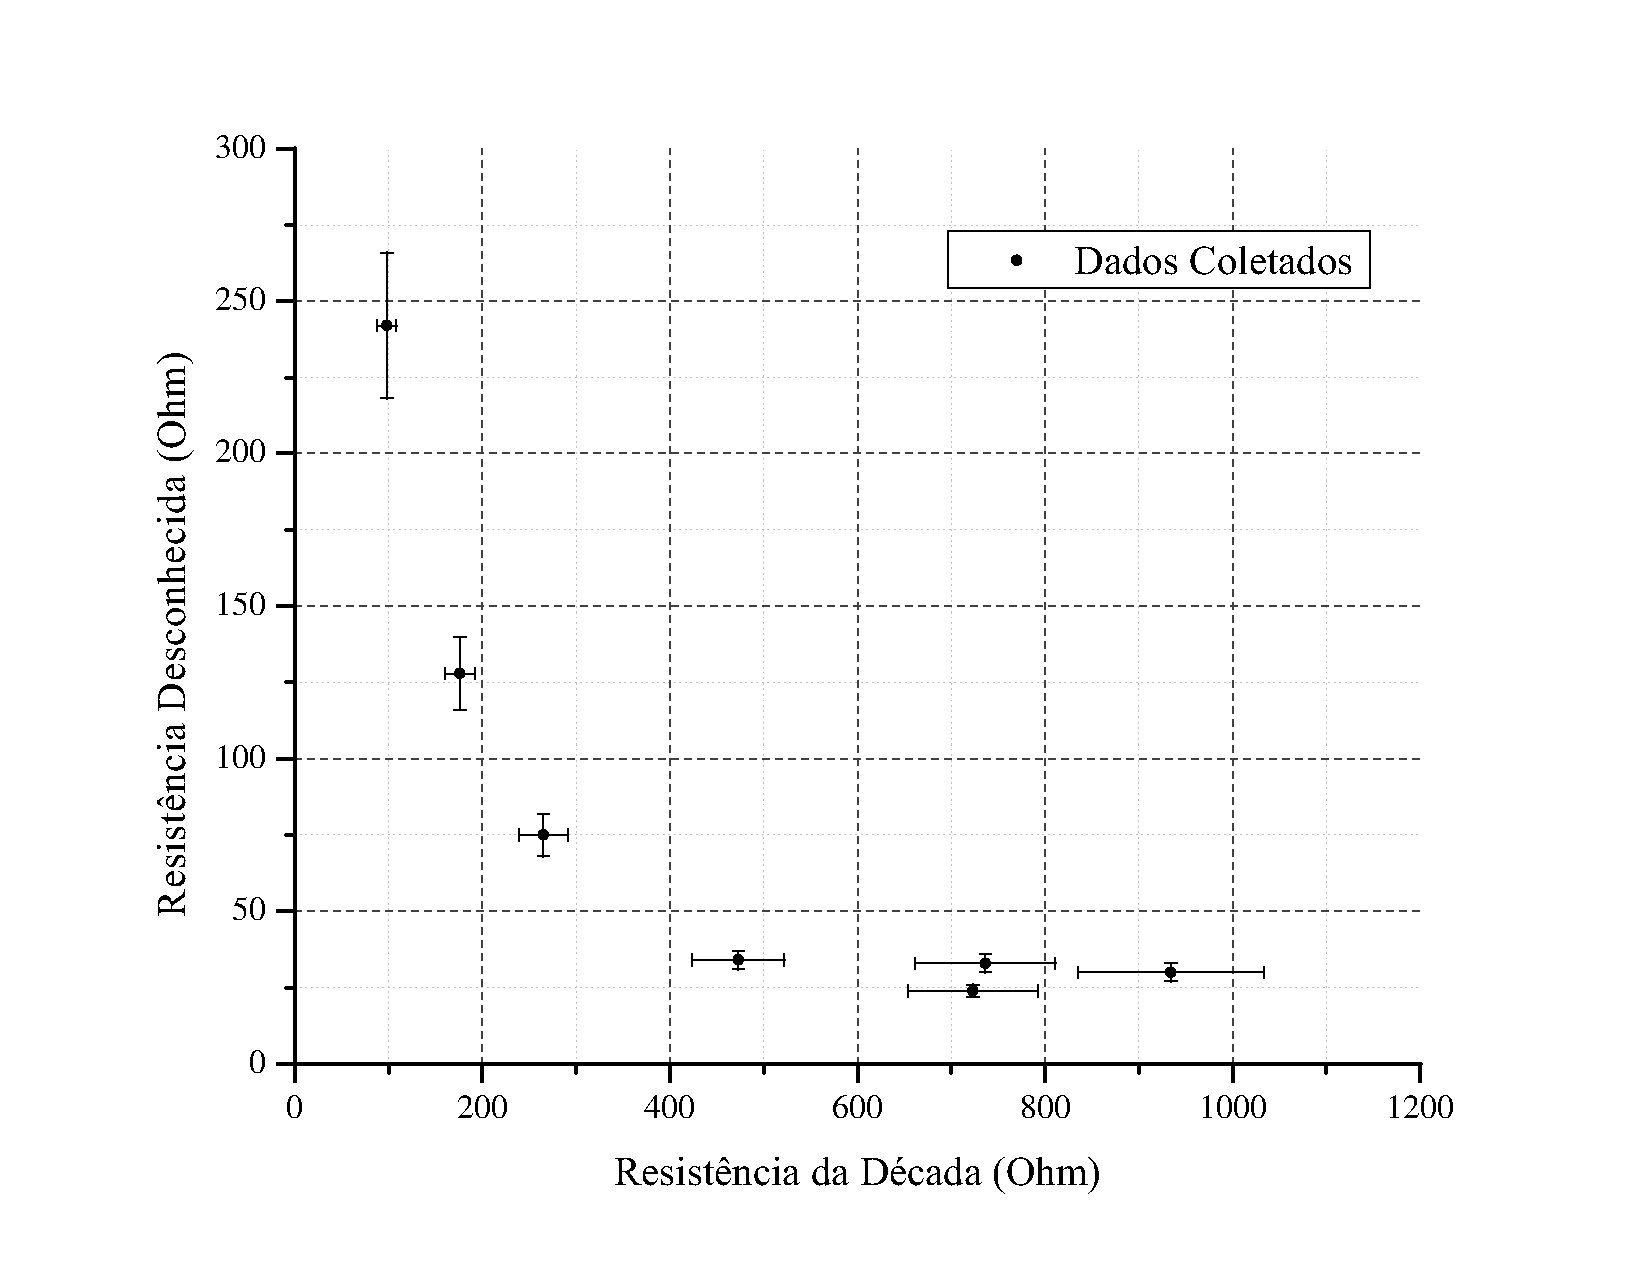
\includegraphics[width=0.6\textwidth]{escala/1dados.pdf}

        \caption{Gráfico da relação da ponte de Wheatstone (\ref{eq:wheatstone})}
        \label{fig:escala:loglog:dados}
    \end{figure}

    \begin{equacao} \label{eq:wheatstone}
        R_x = \frac{R_1 R_2}{R_d}
    \end{equacao}

    Se imaginarmos os dados do gráfico \ref{fig:escala:loglog:dados} como parte de um caso da ponte de Wheatstone dado pela equação \ref{eq:wheatstone}, sendo $R_d$ a resistência da década e $R_x$ a resistência desconhecida, podemos aplicar a seguinte técnica de linearização:

    \begin{align*}
        \log(R_x)
            &= \log\left(R_1 R_2 ~ (R_d)^{-1}\right) \\
            &= \log(R_1 R_2) + \log\left((R_d)^{-1}\right) \\
            &= \log(R_1 R_2) - \log(R_d)
    \end{align*}

    Portanto, podemos montar um gráfico \texttt{log-log} de $R_x$ por $R_d$, cujo coeficiente angular deveria resultar em $-1$.

    \begin{lembrete}
        Cuidado com o posicionamento dos dados na escala logarítmica. Normalmente quando se muda a escala, os ponto mudam de posição em suas novas representações no gráfico e apresentação dos dados pode ser prejudicada. Para atualizar essas posições, o método mais simples é permitir a mudança automática dos limites do gráfico (como na figura \ref{fig:escala:rescale}) e alterar alguma célula da tabela, servindo apenas um simples "copiar e colar" do valor que estava na célula.
    \end{lembrete}

    \begin{figure}[htbp]
        \centering
        \begin{subfigure}{0.45\textwidth}
            \centering
            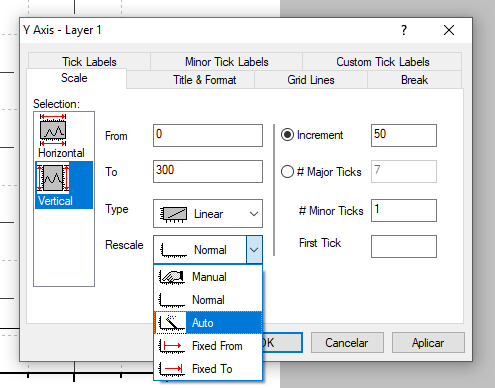
\includegraphics[width=\textwidth]{escala/2rescale.png}

            \caption{Mudança automática dos limites do gráfico}
            \label{fig:escala:rescale}
        \end{subfigure}
        ~
        \begin{subfigure}{0.45\textwidth}
            \centering
            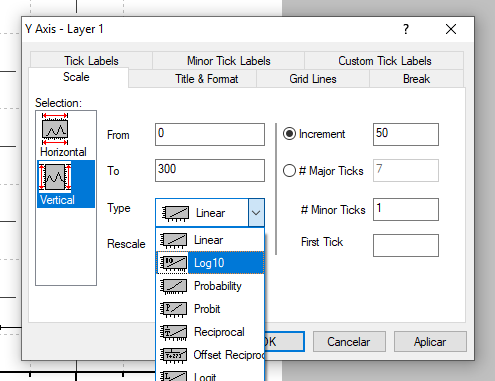
\includegraphics[width=\textwidth]{escala/3logscale.png}

            \caption{Escala logarítmica de base 10}
            \label{fig:escala:logscale}
        \end{subfigure}
        \caption{Colocando a escala logarítmica}
        \label{fig:escala:tutorial}
    \end{figure}

    \begin{figure}[htbp]
        \centering
        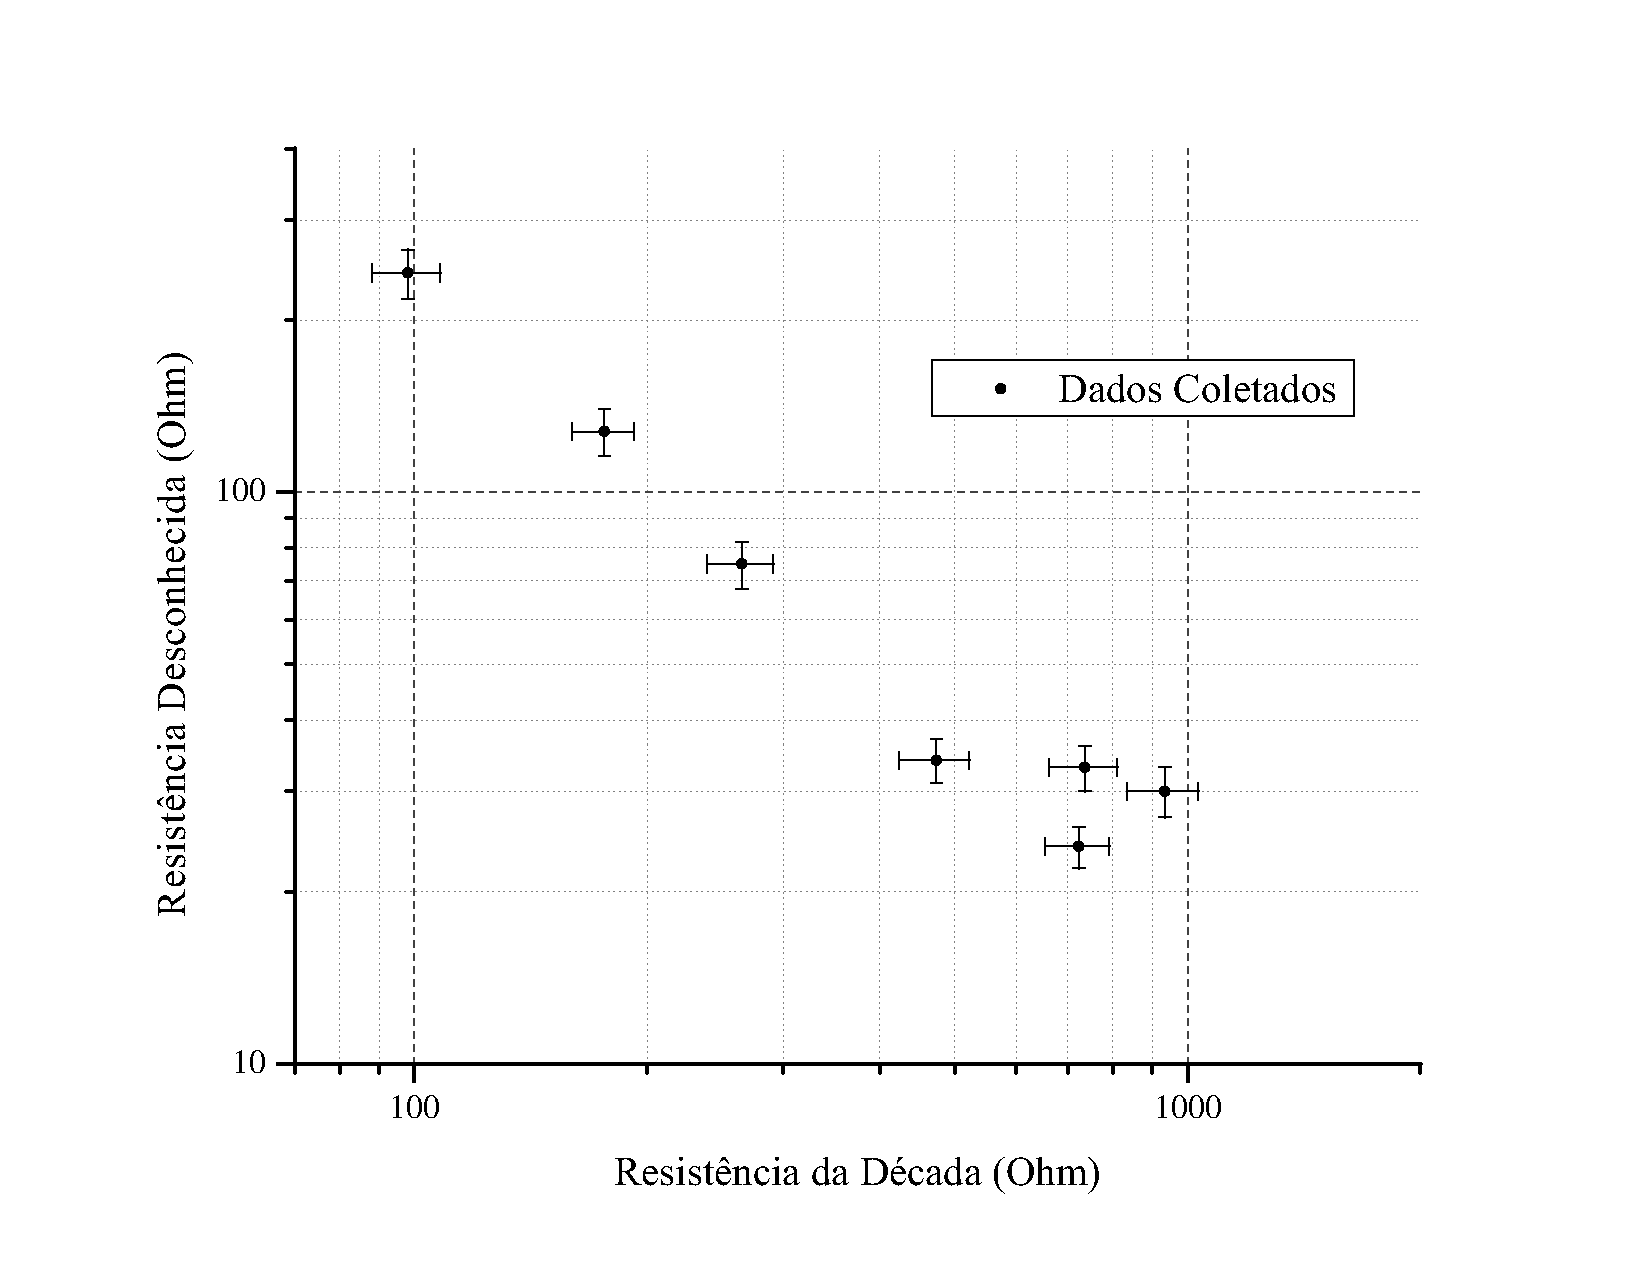
\includegraphics[width=0.8\textwidth]{escala/4loglog.pdf}

        \caption{Gráfico \texttt{log-log} dos dados da figura \ref{fig:escala:loglog:dados}}
        \label{fig:escala:loglog:resultado}
    \end{figure}


\subsection{Gráfico Semi-Log}

    \begin{figure}[htbp]
        \centering
        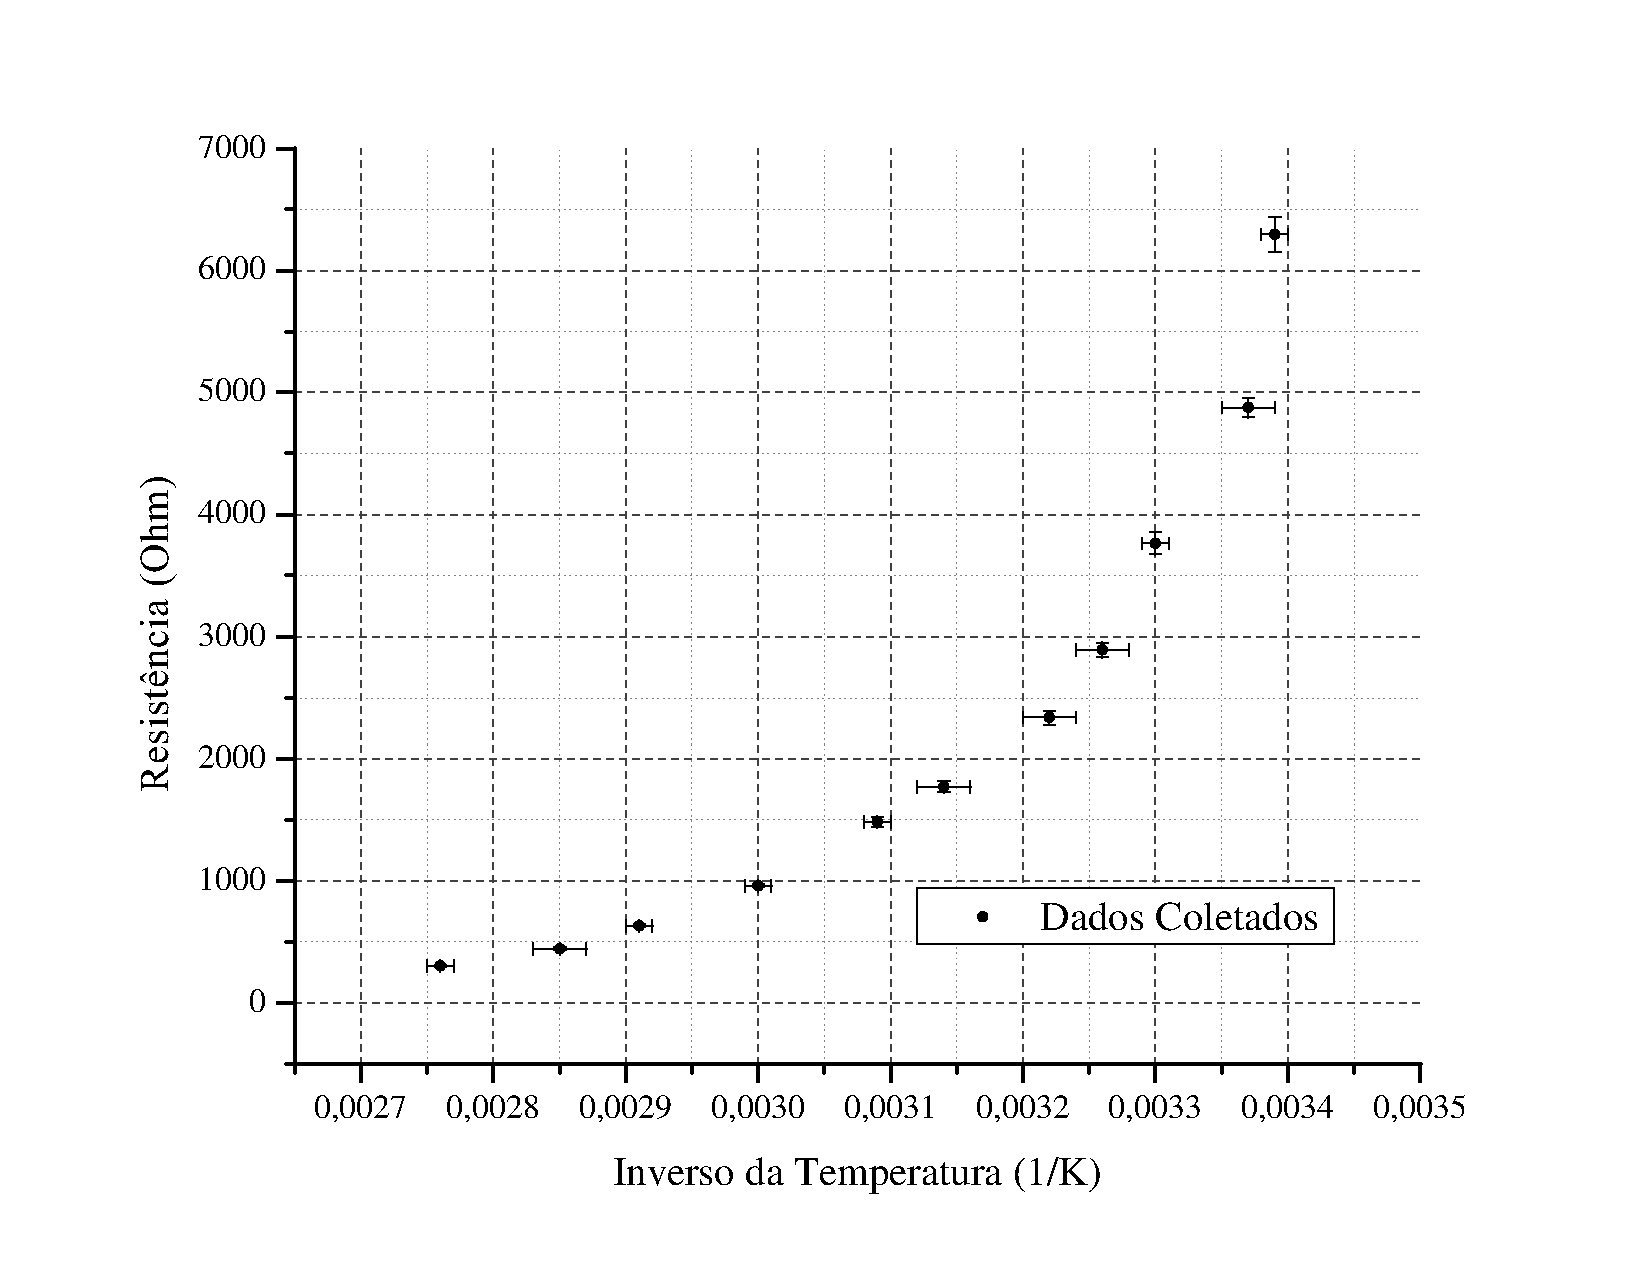
\includegraphics[width=0.6\textwidth]{escala/5dados.pdf}

        \caption{Gráfico da relação (\ref{eq:termistor}) do termistor}
        \label{fig:escala:semilog:dados}
    \end{figure}

    \begin{equacao} \label{eq:termistor}
        R = A ~ \exp\left(B ~ T^{-1}\right)
    \end{equacao}

    Agora com os dados da figura \ref{fig:escala:semilog:dados} e a relação (\ref{eq:termistor}), com $R$ como a resistência e $T^{-1}$ o inverso da temperatura, a linearização se torna:

    \begin{align*}
        \ln(R)
            &= \ln\left(A ~ \exp\left(B ~ T^{-1}\right) \right) \\
            &= \ln(A) + \ln\left(\exp\left(B ~ T^{-1}\right) \right) \\
            &= \ln(A) + B ~ T^{-1}
    \end{align*}

    Que pode ser usada em um gráfico \texttt{semi-log} de $R \times T^{-1}$, como na figura \ref{fig:escala:tutextra}.

    \begin{figure}[htbp]
        \centering
        \begin{subfigure}{0.45\textwidth}
            \centering
            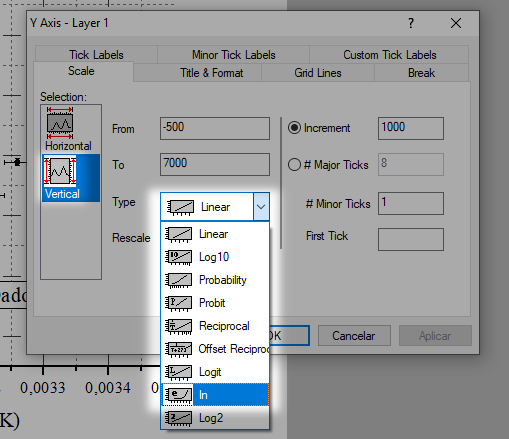
\includegraphics[width=\textwidth]{escala/6lnscale.png}

            \caption{Escala logarítmica de base $e$}
            \label{fig:escala:lnscale}
        \end{subfigure}
        ~
        \begin{subfigure}{0.45\textwidth}
            \centering
            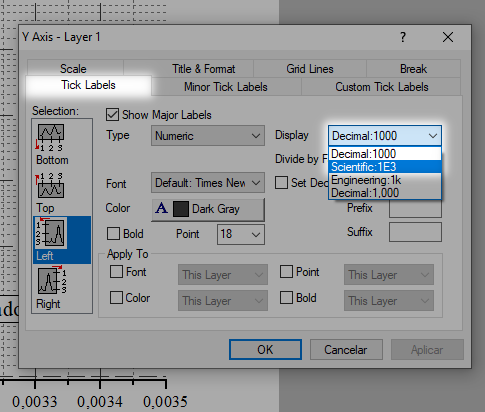
\includegraphics[width=\textwidth]{escala/7expticks.png}

            \caption{Marcadores de escala como expoentes de $e$}
            \label{fig:escala:expticks}
        \end{subfigure}
        \caption{Ajustes para a escala \texttt{ln}}
        \label{fig:escala:tutextra}
    \end{figure}

    \begin{figure}[htbp]
        \centering
        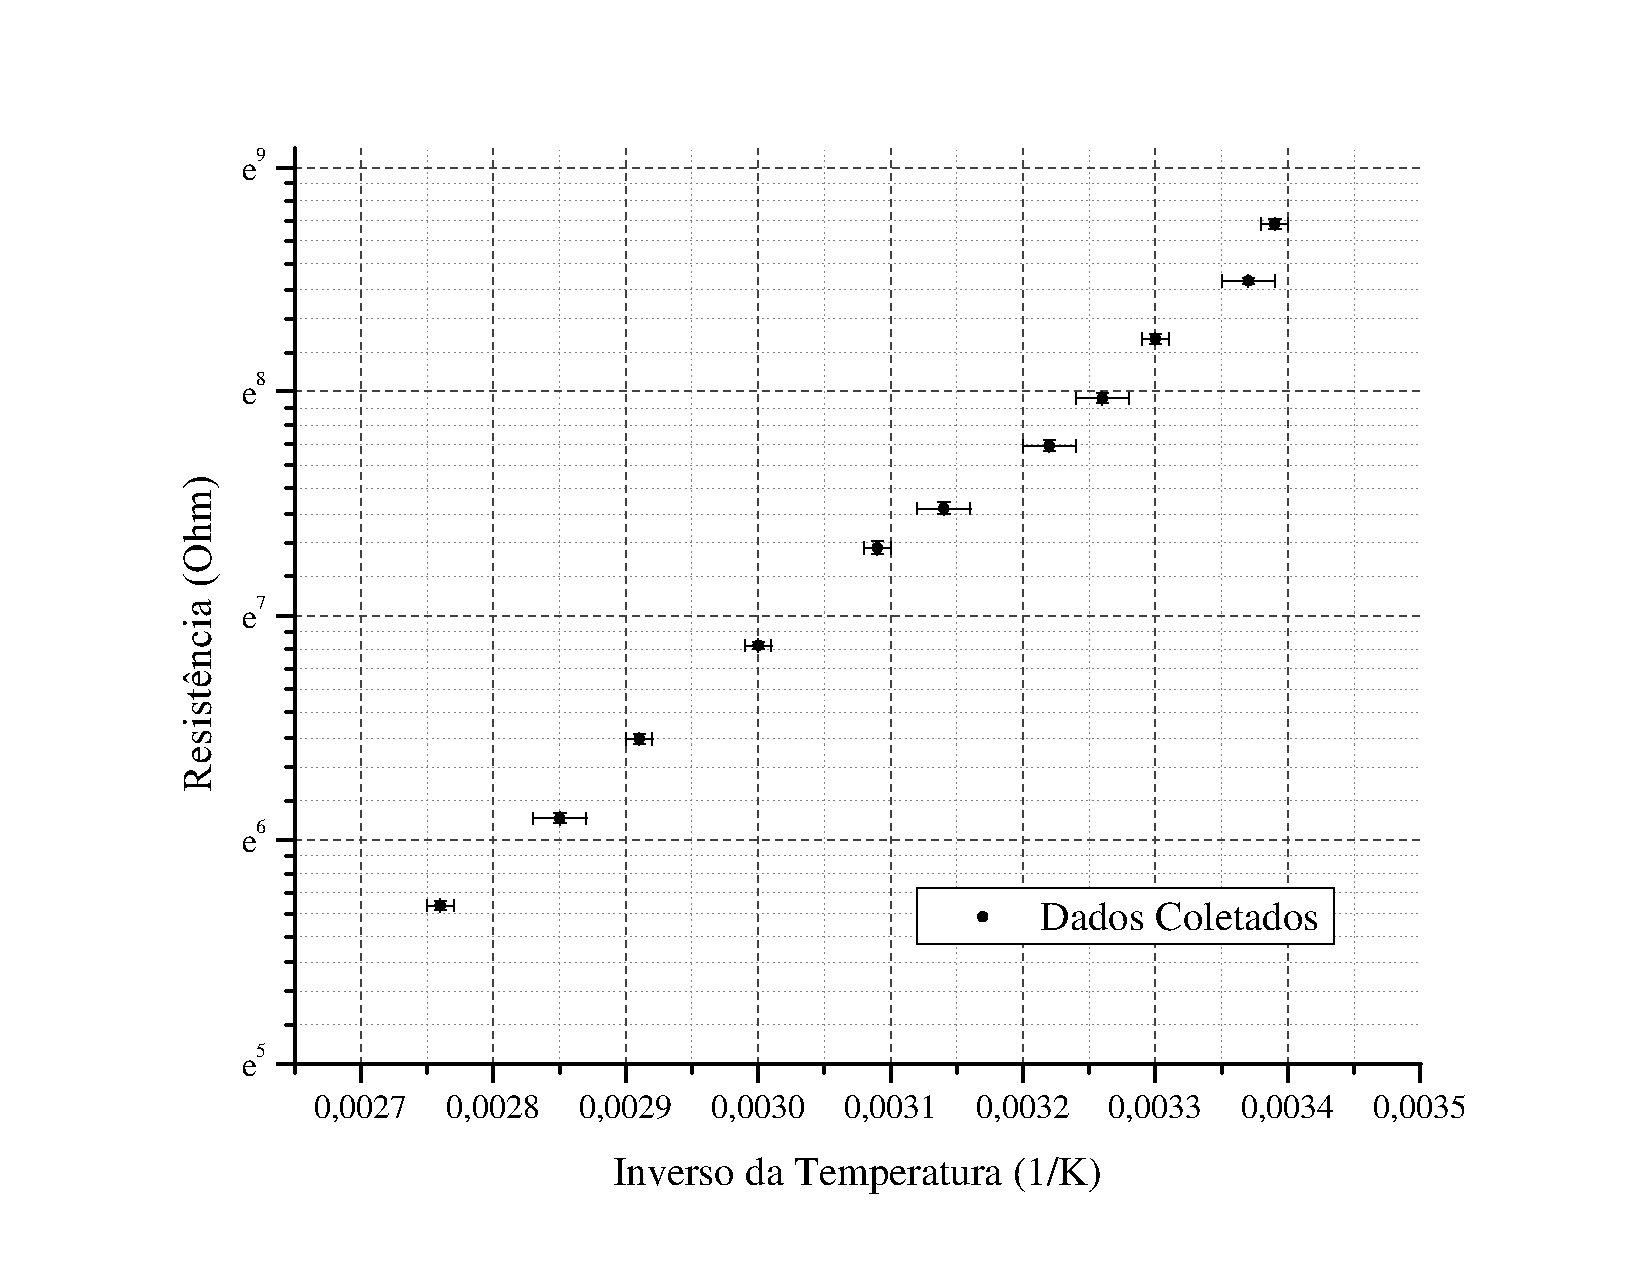
\includegraphics[width=0.8\textwidth]{escala/8semilog.pdf}

        \caption{Gráfico \texttt{semi-log} dos dados da figura \ref{fig:escala:semilog:dados}}
        \label{fig:escala:semilog:resultado}
    \end{figure}


\subsection{Regressão em Escala Logarítmica}

    A regressão de uma curva de potência ou exponencial é possível com técnicas de regressão não-linear, só que essas técnicas não cabem no escopo dessa matéria. Uma outra opção muito utilizada é encontrar uma linearização, como na equação (\ref{eq:linearizacao}), e, com a nova relação linear de $f(x, y) \times g(x, y)$, aplicar a regressão linear como da seção \nameref{sec:regres}. O único detalhe é que é preciso encontrar os valores de $f(x, y)$ e $g(x, y)$ e suas incertezas para cada par $(x, y)$ dos dados e só com esses valores pode-se encontrar os coeficientes $a$ e $b$, como foi feito na figura \ref{fig:escala:regres}.

    \begin{figure}[htbp]
        \centering
        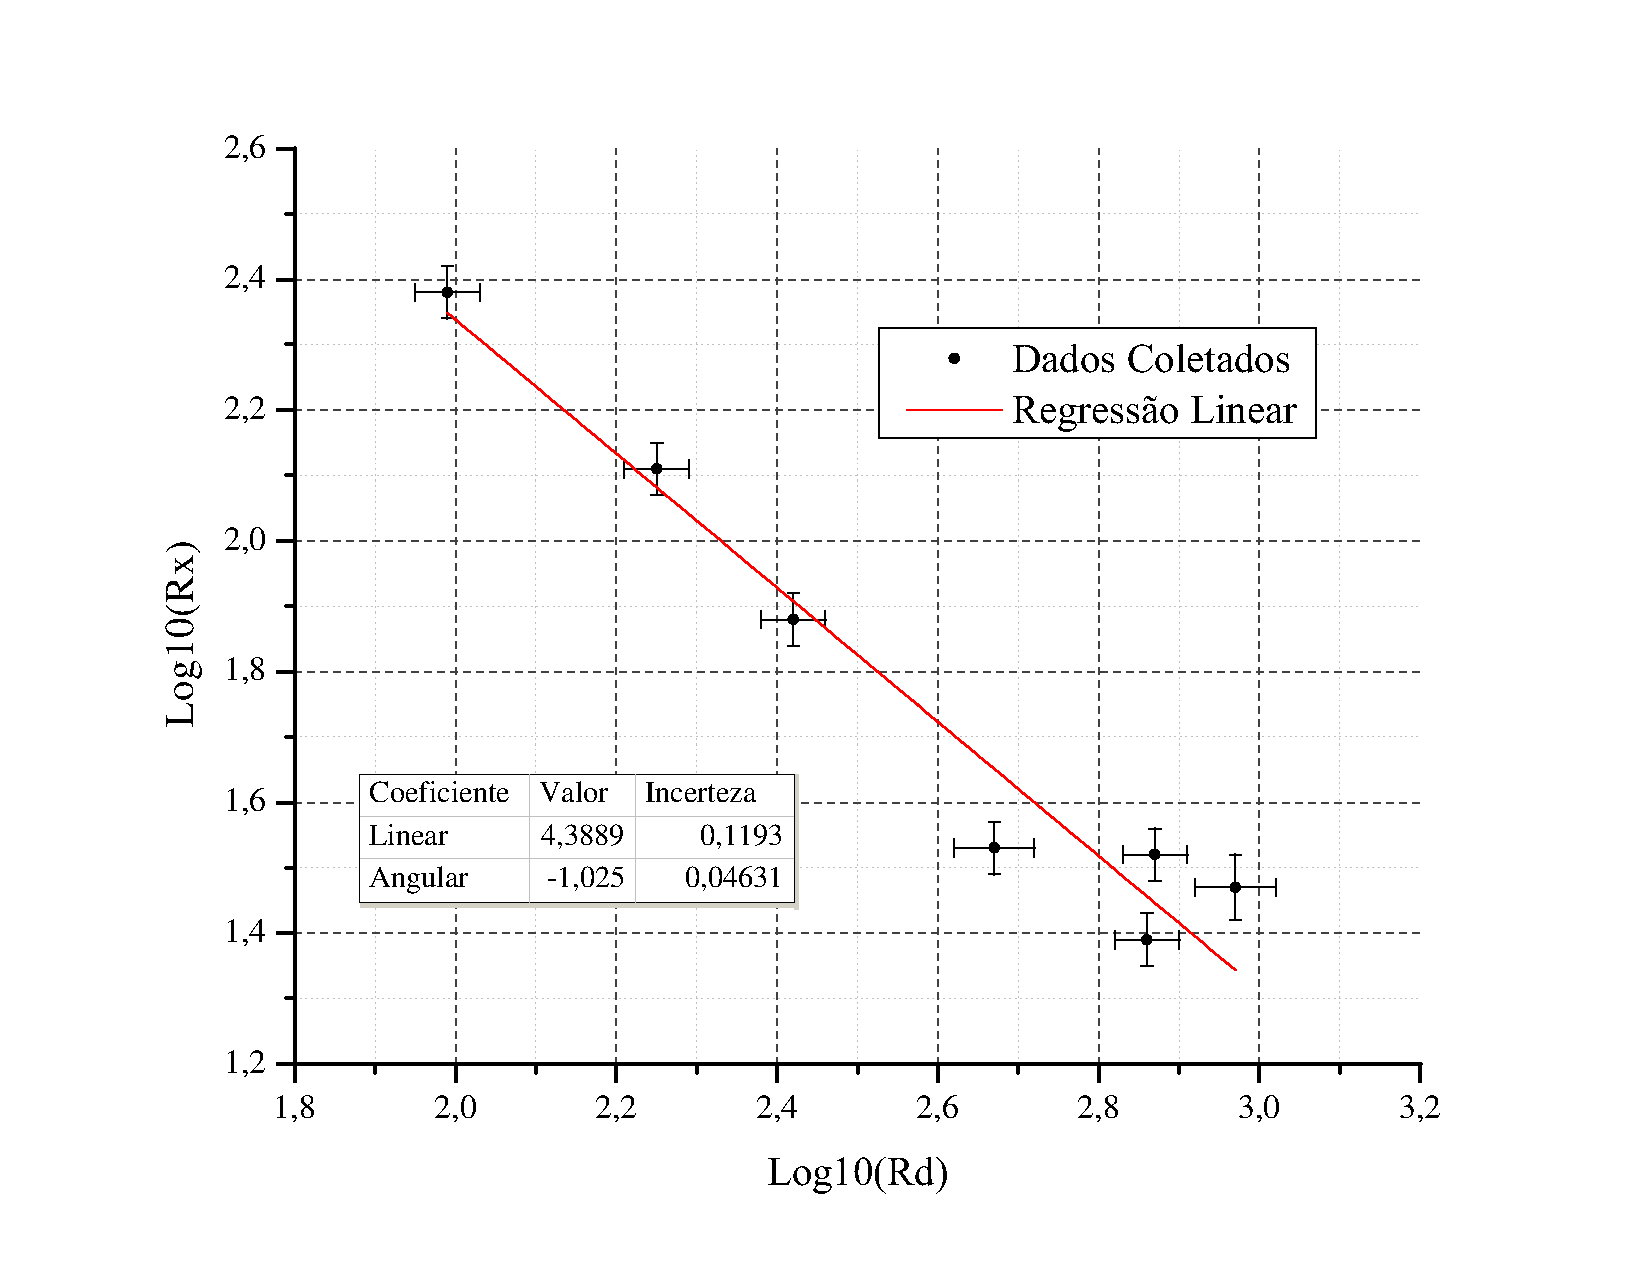
\includegraphics[width=0.8\textwidth]{escala/9logreg.pdf}

        \caption{Gráfico da regressão da relação (\ref{eq:wheatstone}). Isso seviria para mostrar que $b \approx -1$, por exemplo.}
        \label{fig:escala:regres}
    \end{figure}

    A mudança dos dados de $(x, y)$ para $(f(x, y), g(x, y))$ ajuda nos cálculos, só que normalmente causa um distanciamento do sentido físco dos dados. Então, é importante decidir qual dos gráficos utilizar ou se cabe usar os dois gráficos.


    \section{Curva Característica} \label{sec:caract}
        Um exemplo de equação característica é a equação (\ref{eq:termistor}), do termistor, que será utilizada nesta seção. Os dados gerados para o gráfico \ref{fig:escala:semilog:dados} continuarão os mesmos aqui.

\subsection{Encontrando os Coeficientes}

    O primeiro passo normalmente é encontrar os coeficientes da equação característica. Se for uma equação de reta, uma simples regressão linear é bastante para encontrar esses coeficientes e para mostrar a equação esperada. Para os outros caso, no entanto, é preciso linearizar a equação, como foi feito na seção \nameref{sec:escala}, encontrar os coeficientes da linearização e transformar para os coeficientes da equação inicial.

    No caso dos dados do termistor, a regressão é aplicada como na figura \ref{fig:caract:regres}. Logo, os coeficientes se tornam $A = \exp(-7.07097) \approxeq 0.00084941$ e $B = 4632.762$.

    \begin{figure}[htbp]
        \centering
        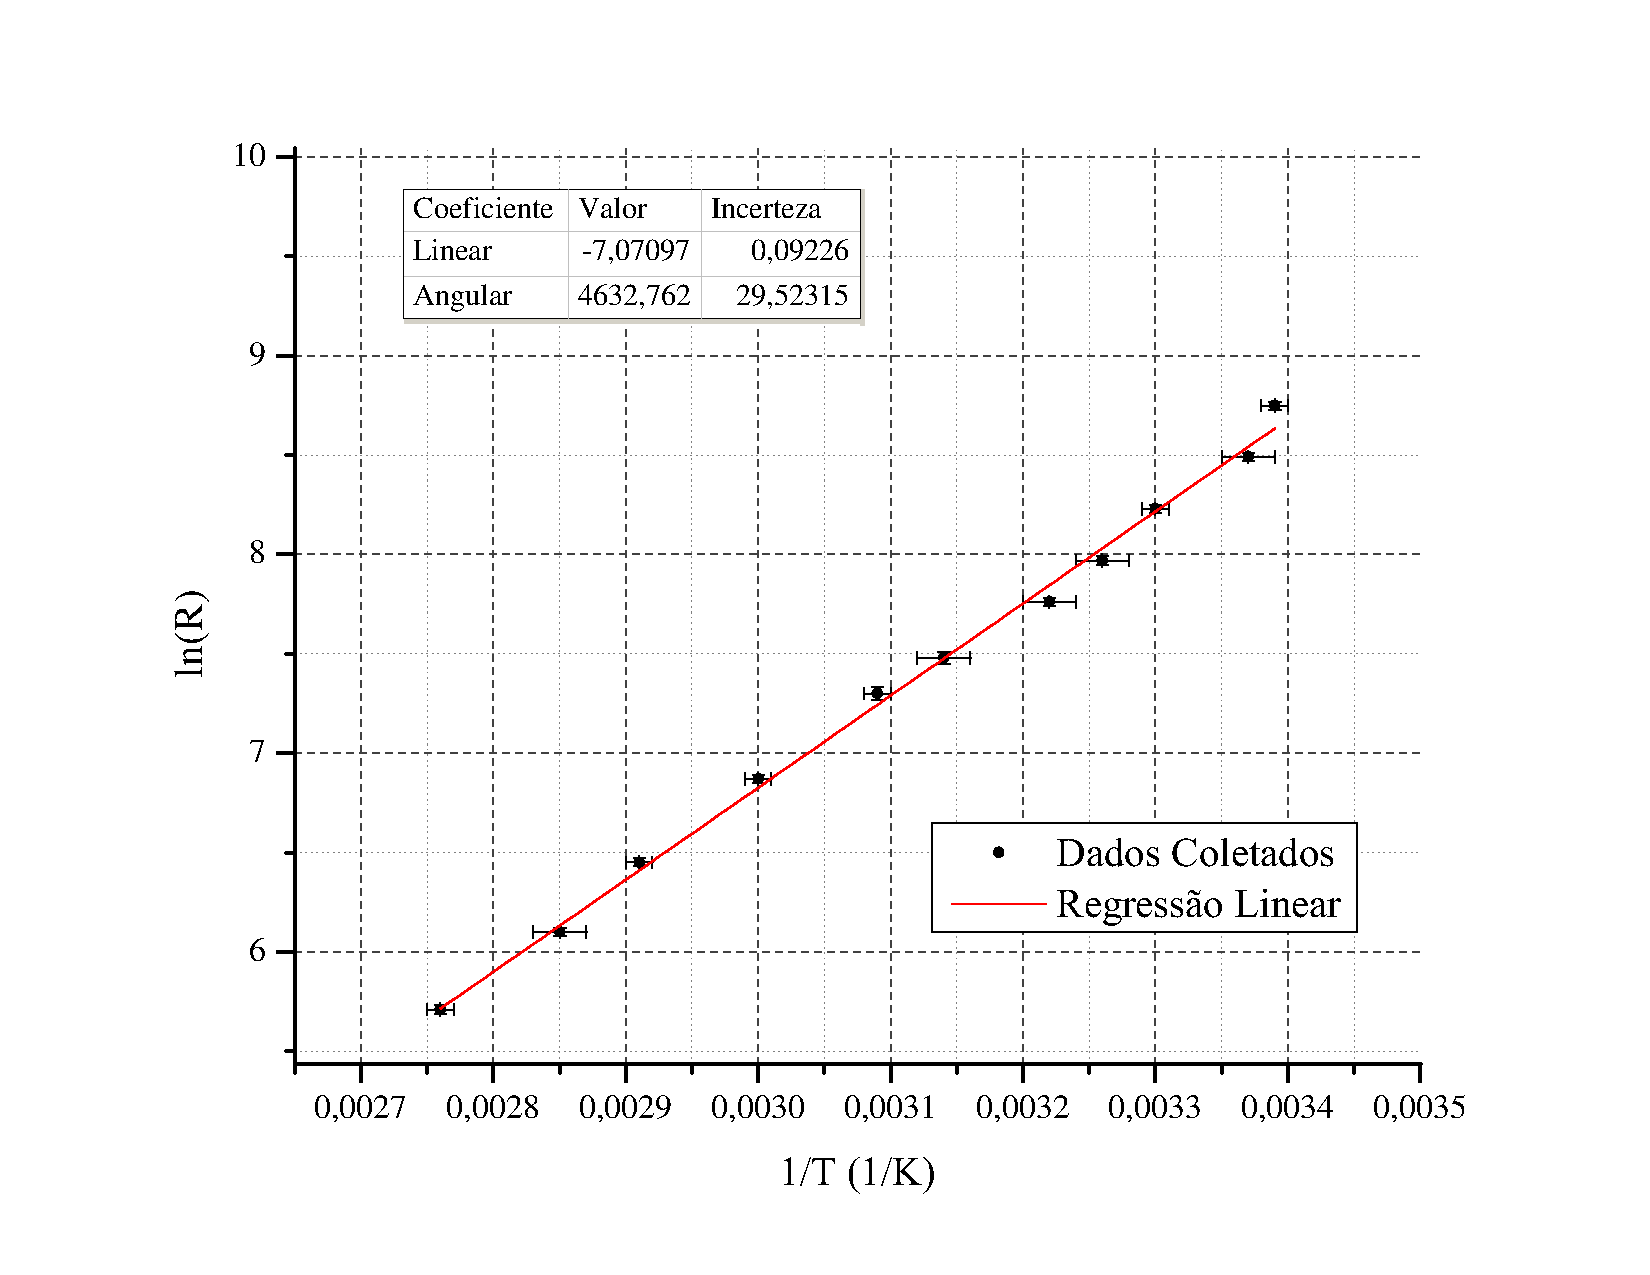
\includegraphics[width=0.8\textwidth]{caract/1regres.pdf}

        \caption{Gráfico da linearização da equação (\ref{eq:termistor})}
        \label{fig:caract:regres}
    \end{figure}


    \subsection{Gráfico de Funções}

    Voltando para os dados originais, de $R$ por $T$, podemos desenhar a equação característica, agora com os valores dos coeficientes, sobre o \texttt{Scatter} dos dados, como mostra a figura \ref{fig:caract:inserir}.

    \begin{figure}[htbp]
        \centering
        \begin{subfigure}{0.32\textwidth}
            \centering
            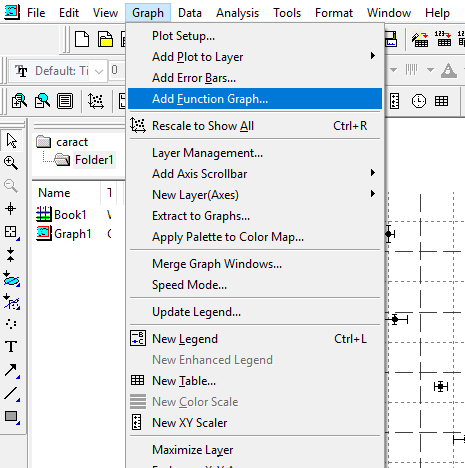
\includegraphics[width=\textwidth]{caract/2insert.png}

            \caption{Adicionando uma função no gráfico}
            \label{fig:caract:novo}
        \end{subfigure}
        ~
        \begin{subfigure}{0.63\textwidth}
            \centering
            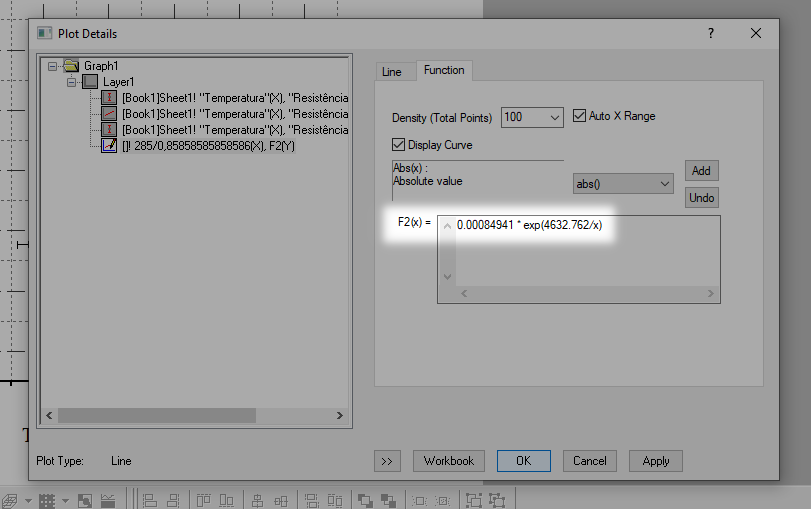
\includegraphics[width=\textwidth]{caract/4funcao.png}

            \caption{Colocando a função $R = 0.00084941 ~ \exp(4632.762/T)$}
            \label{fig:caract:funcao}
        \end{subfigure}
        \caption{Desenhando uma função no gráfico}
        \label{fig:caract:inserir}
    \end{figure}


\subsection{Ajustes de Formatação}

    Por padrão, a cor da nova curva do gráfico é escolhida como preto, mas isso pode ser mudado com um duplo clique sobre a curva. Neste exemplo a cor decidida foi vermelho, que acompanha o padrão de regressão dos exemplos anteriores.

    \begin{figure}[htbp]
        \centering
        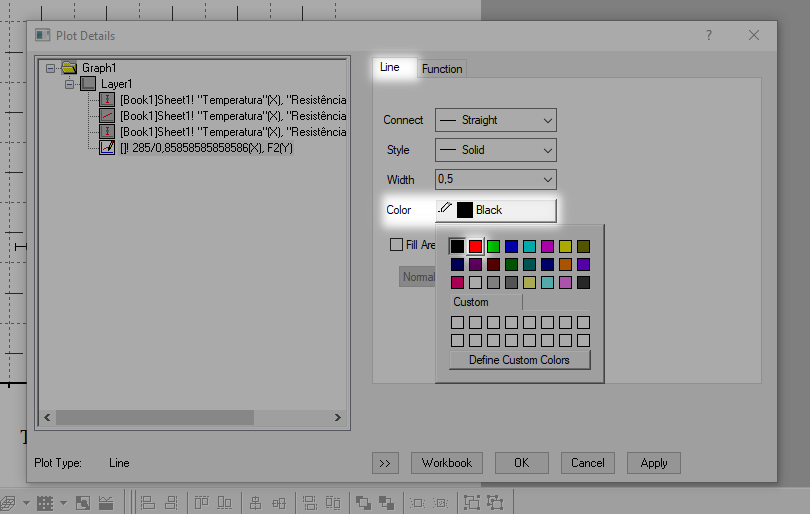
\includegraphics[width=0.8\textwidth]{caract/5cor.png}

        \caption{Mudança da cor da nova curva}
        \label{fig:caract:cor}
    \end{figure}

    Além da cor, é importante lembrar de tratar da curva na legenda do gráfico, caso isso não tenha sido feito automaticamente, que pode ser feito pelas propriedades da legenda. Normalmente, a descrição da curva pode ser dada também pela sua forma algébrica.

    \begin{figure}[htbp]
        \centering
        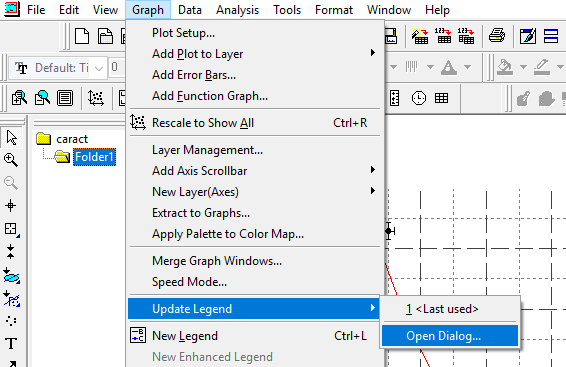
\includegraphics[width=0.7\textwidth]{caract/6leg.png}
        \caption{Atualizando a legenda com a nova curva}
        \label{fig:caract:legenda}
    \end{figure}


\subsection{Resultado}

    \begin{figure}[htbp]
        \centering
        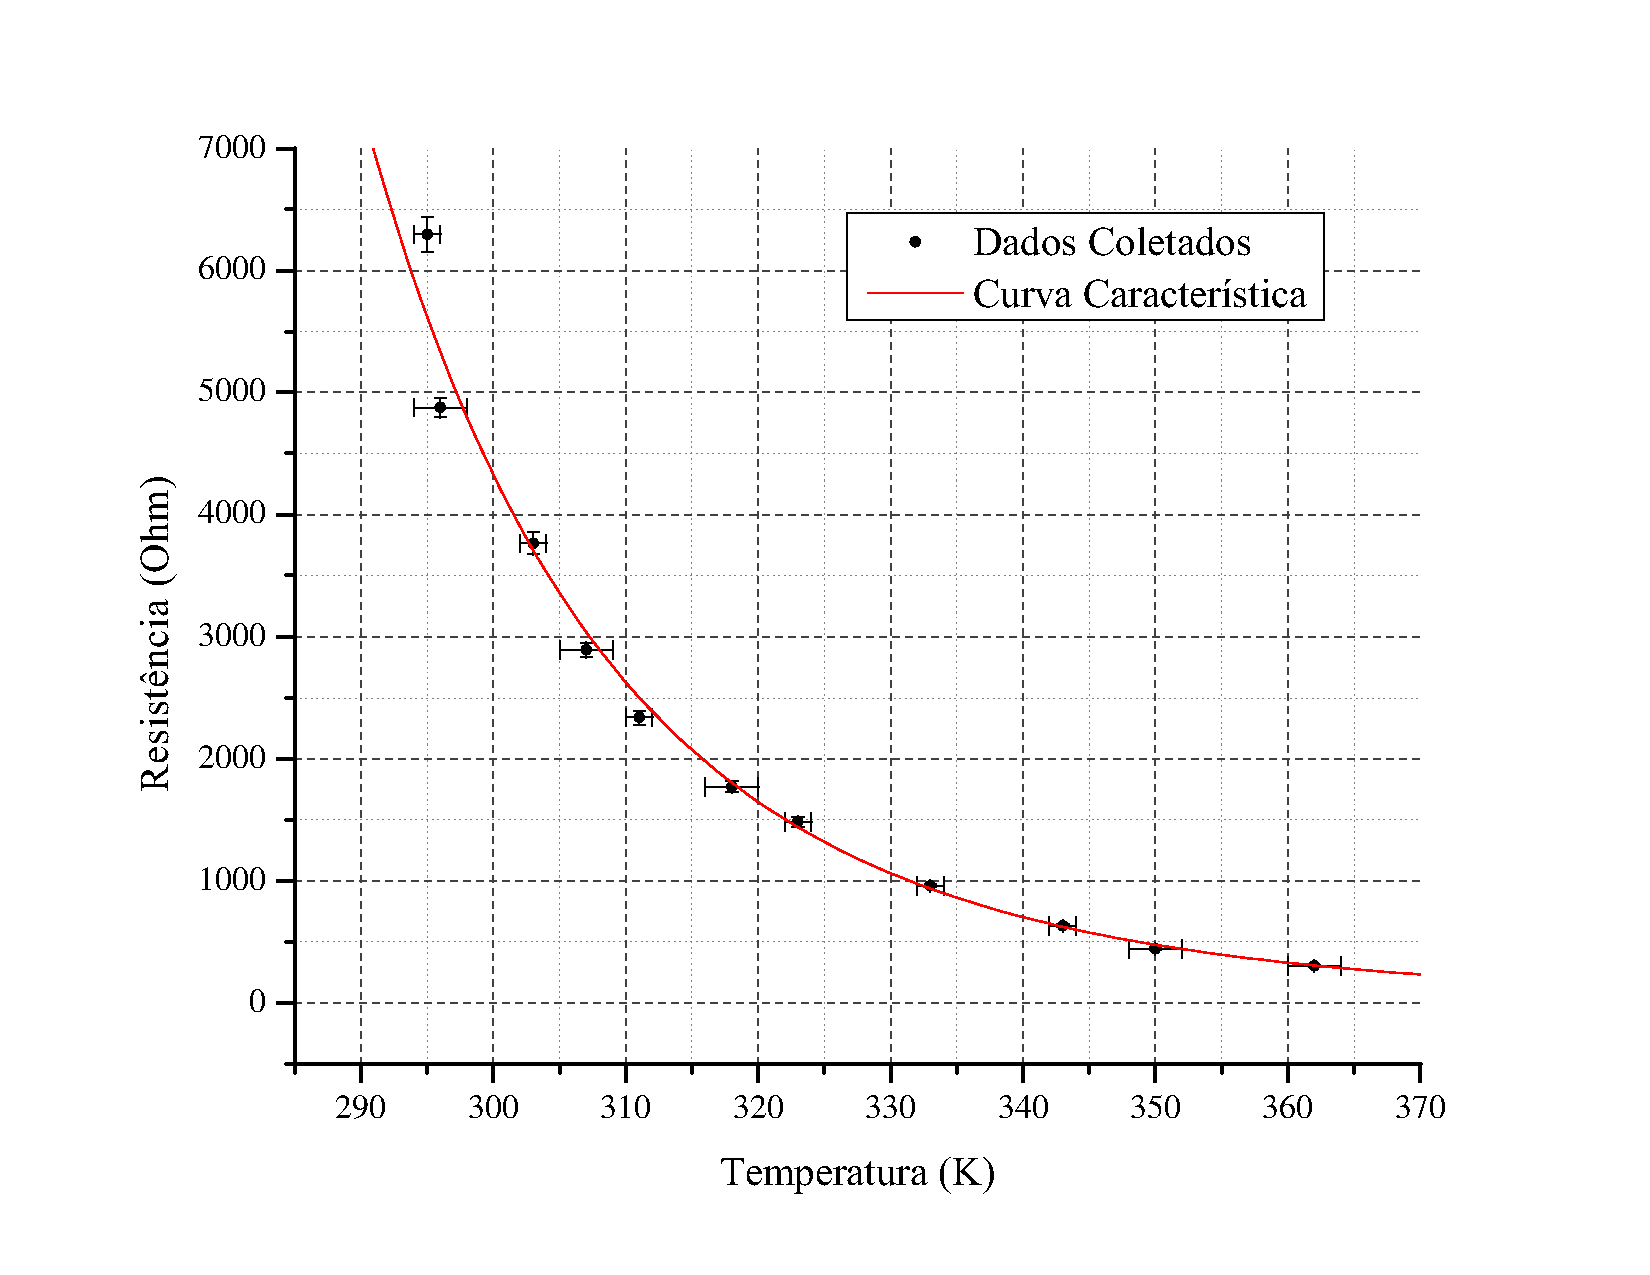
\includegraphics[width=0.8\textwidth]{caract/8final.pdf}

        \caption{Gráfico com a curva característica do termistor}
        \label{fig:caract:final}
    \end{figure}


    \section{Gráficos de Múltiplas Variáveis} \label{sec:multiv}
        \edef\indentacao{\the\parindent}

\noindent
\begin{minipage}[t]{0.55\textwidth}\setlength{\parindent}{\indentacao}

    Para os casos em que é necessário apresentar dados com mais de uma váriavel dependente de um mesmo \texttt{X}, existe a opção de gráficos múltiplos. Eles servem para comparar as relações do tipo $y_1 = f(x)$ e $y_2 = g(x)$, quando $x$, $y_1$ e $y_2$ são medidos em conjunto.

    Em experimentos com circuitos, esse tipo de dado aparece, por exemplo, na medição de tensão em nós diferentes para a comparação de seus comportamentos no tempo. É o caso do circuito da figura \ref{fig:multiv:circuito}, cujos dados foram colocados como na figura \ref{fig:multiv:dados}.

    \begin{figure}[H]
        \centering
        \includegraphics[width=0.8\textwidth]{multiv/1dados.png}

        \caption{Dados gerados com simulador}
        \label{fig:multiv:dados}
    \end{figure}

\end{minipage}\vspace{0.05\textwidth}%
\begin{minipage}[t]{0.4\textwidth}
    \begin{figure}[H]
        \centering
        \begin{circuitikz}[scale=1.2]

    \draw (2, 0)
    to [short] ++(-2,0)
    to [vsourcesin, l=$E$] ++(0,4)
    to [short] ++(2,0)
    to [resistor, l_=$R$] ++(0,-2)
    to [capacitor, l_=$C$] ++(0,-2)
    node[ground] {};

    \draw [->, thick] (3,4) to node[above] {$V_1$} (2.1,4);

    \draw [->, thick] (3,2) to node[above] {$V_2$} (2.1,2);

\end{circuitikz}


        \caption{Circuito com defasagem de tensão por um capacitor}
        \label{fig:multiv:circuito}
    \end{figure}
\end{minipage}


\subsection{Gráficos de Eixos Separados}

    Uma opção para mostrar os dois canais ao mesmo tempo é colocar cada um em seu próprio gŕafico com seus próprios eixos. No \software, isso é feito como na figura \ref{fig:multiv:paneis:tutorial}, mas pode ser feito em duas imagens separadas também. O problema com essa abordagem é que as escalas diferentes não mostram muito bem as proporções entre os canais de entrada e saída.

    \begin{figure}[H]
        \centering
        \includegraphics[width=0.6\textwidth]{multiv/2paneis.png}

        \caption{Criando os gráficos separados}
        \label{fig:multiv:paneis:tutorial}
    \end{figure}

    \begin{figure}[H]
        \centering
        \includegraphics[width=0.8\textwidth]{multiv/3paneis.pdf}

        \caption{Gráficos das tensões de entrada e saída do circuito}
        \label{fig:multiv:paneis}
    \end{figure}


\subsection{Gráficos de Eixos em Conjunto}

    \begin{figure}[htbp]
        \centering
        \includegraphics[width=0.6\textwidth]{multiv/4dois.png}

        \caption{Criando o gráfico com as duas curvas}
        \label{fig:multiv:juntos:tutorial}
    \end{figure}

    \noindent
    \begin{minipage}[t]{0.35\textwidth}
        \begin{figure}[H]
            \centering
            \includegraphics[width=\textwidth]{multiv/5dois.png}

            \caption{Formatação do rótulo dos eixos}
            \label{fig:multiv:juntos:formatacao}
        \end{figure}
    \end{minipage}\hspace{0.05\textwidth}%
    \begin{minipage}[t]{0.6\textwidth}\setlength{\parindent}{\indentacao}

        Quando o gráfico é criado como na figura \ref{fig:multiv:juntos:tutorial}, o rótulo do eixo $y$ fica como o nome de apenas uma das colunas dos dados. Pra consertar isso basta alterar o nome do eixo para algum texto que descreve ambas variáveis (figura \ref{fig:multiv:juntos:formatacao}).

        Um dos maiores limites para esse método é que as variáveis dependentes precisam ter a mesma motivação física e, por causa disso, a mesma gradeza, caso contrário, o eixo compartilhado entre elas perde completamente o sentido.

    \end{minipage}

    \begin{figure}[htbp]
        \centering
        \includegraphics[width=0.8\textwidth]{multiv/6dois.pdf}

        \caption{Gráfico das tensões $V_1$ e $V_2$ do circuito}
        \label{fig:multiv:juntos}
    \end{figure}


\subsection{Gráficos com Apenas a Abscissa Comum}

    \begin{figure}[htbp]
        \centering
        \includegraphics[width=0.6\textwidth]{multiv/7duplo.png}

        \caption{Criando o gráfico com três eixos}
        \label{fig:multiv:duplo:tutorial}
    \end{figure}

    Imagine agora o caso em que queremos mostrar a defasagem entre a corrente a tensão no capacitor da figura \ref{fig:multiv:circuito}. A única grandeza comum agora é o tempo, então vamos precisar de gráficos de três eixos. No \software, isso é feito como mostra a imagem \ref{fig:multiv:duplo:tutorial}. Normalmente, é melhor alterar as cores para melhor representar cada dado.

    \begin{figure}[htbp]
        \centering
        \includegraphics[width=0.8\textwidth]{multiv/8duplo.pdf}

        \caption{Gráfico de corrente e tensão em um capacitor por tempo}
        \label{fig:multiv:duplo}
    \end{figure}

    \begin{nota}
        As vezes, os gráficos com múltiplas curvas podem ficar sobrecarregado de informação. Quando isso acontece, o melhor é separar os dados em gráficos distintos pra manter a legibilidade. Gráficos de três eixos podem ficar complicados com facilidade.
    \end{nota}


    \section{Curvas de Nível} \label{sec:contorno}
        Curvas de nível servem para representar dados tridimensionais em um plano. As três variáveis para esse tipo de gráfico são $x$ e $y$ independentes e $z = f(x,y)$.

Serão usados, como exemplo, dados semelhantes aos do experimento sobre potencial elétrico entre barras de cobre em uma solução condutiva. Nesse caso, as variáveis dependentes são as distâncias $x$ e $y$ no plano e a variável dependente é o potencial $V$ de cada ponto.

\begin{figure}[htbp]
    \centering
    \includegraphics[width=0.4\textwidth]{contorno/1dados.png}

    \caption{Montagem dos dados de potencial na tabela do \software}
    \label{fig:contorno:dados}
\end{figure}


\subsection{Iniciando o Gráfico}

    \begin{figure}[htbp]
        \centering
        \includegraphics[width=0.8\textwidth]{contorno/2plot.png}

        \caption{Desenhando o gráfico de linhas de contorno}
        \label{fig:contorno:plot}
    \end{figure}

\subsection{Opções de Formatação}

    \begin{figure}[H]
        \centering
        \begin{subfigure}{0.7\textwidth}
            \centering
            \includegraphics[width=\textwidth]{contorno/4sufixo.png}

            \caption{Adição de um sufixo nos dados em $z$}
            \label{fig:contorno:sufixo}
        \end{subfigure}
        ~
        \begin{subfigure}{0.7\textwidth}
            \centering
            \includegraphics[width=\textwidth]{contorno/6linha.png}

            \caption{Mudança do estilo das linhas de separação dos níveis}
            \label{fig:contorno:linhas}
        \end{subfigure}
        \caption{Opções do gráfico de curvas de nível}
        \label{fig:contorno:opcoes}
    \end{figure}

    \begin{lembrete}
        É importante a adição de sufixos com a unidade do valor medido (figura \ref{fig:contorno:sufixo}).
    \end{lembrete}

    Para as paletas de cores existem muitas opções e vale mais a pena testar qual paleta funciona melhor com os seus dados. A caixa de opções é acessada como na figura \ref{fig:contorno:paleta}. A caixa da figura \ref{fig:contorno:escala} é acessada com um clique duplo na caixa com os níveis do eixo $z$.

    \begin{figure}[H]
        \centering
        \begin{subfigure}{0.45\textwidth}
            \centering
            \includegraphics[width=\textwidth]{contorno/3paleta.png}

            \caption{Mudança da paleta de cores}
            \label{fig:contorno:paleta}
        \end{subfigure}
        ~
        \begin{subfigure}{0.45\textwidth}
            \centering
            \includegraphics[width=\textwidth]{contorno/5bg.png}

            \caption{Opções da escala de níveis}
            \label{fig:contorno:escala}
        \end{subfigure}
        \caption{Mais opções de formatação}
        \label{fig:contorno:extra}
    \end{figure}

\subsection{Resultado}

    \begin{figure}[htbp]
        \centering
        \includegraphics[width=0.9\textwidth]{contorno/resultado.pdf}

        \caption{Deformação das equipotenciais gerada pela adição de uma ponta}
        \label{fig:contorno:final}
    \end{figure}



\end{document}
